%%%%%%%%%%%%%%
% Modelo XXXXXXXXXXXXXXX
% Autor: Leonardo Garcez Dalenogari Alba
% Ano: 2022
% Contato: leonardo.2017007421@aluno.iffar.edu.br

% IMPORTANTE: 
%   O modelo utiliza o compilador XeLaTex (talvez possam ser utilizados outros, mas não é garantido o correto funcionamento, visto que seria necessário testar, porém, eu sei que alguns vão apresentar problemas na hora de compilar, como o pdflatex)
%   Se você estiver utilizando o Overleaf, com o documento aberto, clique em Menu, no canto superior esquerdo, e selecione o XeLaTex como compilador
%   Também é utilizado o biber para gerenciar as referências bibliográficas
%%%%%%%%%%%%%%

\documentclass[
    12pt, % Tamanho de fonte definido para 12, se você precisar utilizar um texto em tamanho 10, utilize o comando \footnotesize, que será impresso em tamanho 10
    oneside, % Essa opção vem ativada por padrão, para imprimir em apenas um lado da folha. Comente esta e descomente a opção de baixo se quiser imprimir nos dois lados de uma folha.
    % twoside, % A opção permite gerar o documento utilizando o verso das páginas, porém, ela não indica à impressora que você está utilizando isso ou que ela deva imprimir nos dois lados das folhas (fonte: https://en.wikibooks.org/wiki/LaTeX/Document_Structure)
    openany,
    % openright, % Essa seria uma opção válida, se não afetasse também os capítulos pós-textuais
    a4paper,
    english,
    brazil
]{report}
% Pacotinho básico só pra garantir que a folha de rosto esteja sempre no anverso do documento (no caso de twoside)
\usepackage{config/onesidetwoside}

% Pacotes que envolvem codificação do conteúdo. Essenciais.
\usepackage[T1]{fontenc}
% \usepackage[utf8]{inputenc} % Não é necessário se você estiver utilizando um compilador LaTeX baseado já em UTF-8

% Responsável pela quebra silábica de palavras no final de linha de forma correta para o português
\usepackage[brazil]{babel}
% O pacote babel recomenda o uso do csquotes, para garantir que textos citados estejam escritos corretamente de acordo com as regras do seu idioma. Mesmo assim foi necessário adaptar para o padrão ABNT.
\usepackage[portuguese=brazilian, style=brazilian]{csquotes}
\usepackage{config/citacao} % As configurações para que as citações longas sigam a ABNT

%% Pacotes para formatação de fonte do documento
\usepackage{fontspec}
% Pode ser Times New Roman:
% \setmainfont{Times New Roman} 
% Ou pode ser Arial, também:
\setmainfont{Arial}

% Pacote responsável por adicionar símbolos matemáticos. Símbolos, por exemplo, também necessários para o correto referenciamento de leis e decretos
\usepackage{amssymb}
% Só que também é importante realizar a configuração para adicionar os comandos que imprimem esses símbolos associados aos caracteres que imprimem, assim, você pode adicionar o símbolo diretamente no texto
\usepackage{newunicodechar} % Pacote que permite definir novos caracteres
\usepackage{config/unicode-char} % Arquivo de configuração com a listagem desses caracteres

%% Pacotes para formatação de conteúdo na página
\usepackage[left=3cm,top=3cm,right=2cm,bottom=2cm]{geometry} % Pacote responsável por formatar as dimensões das margens das páginas.
\usepackage{setspace} % Adiciona opções de espaçamento de texto
\usepackage[skip=1.241pt, indent=1.25cm]{parskip} % O recomendado é utilizar esse pacote para gerenciar o parskip e o parindent, ao invés de definir as unidades manualmente no documento, que pode levar a problemas de formatação
\usepackage{ragged2e} % Adiciona opções mais completas para alinhamento de texto
\usepackage{indentfirst} % Faz com que o primeiro parágrafo de cada seção possua indentação também

% Pacote que permite criar estilos para o cabeçalho
\usepackage{fancyhdr}
\usepackage{config/cabecalho} % Cabeçalho customizado para o modelo

%% Adiciono os pacotes para configurar e estilizar o sumário e as seções
\usepackage{titletoc}
\usepackage{titlesec}
\usepackage{alphalph} % Permite lidar com contadores que possuam valor maior que 26 utilizando o alfabeto (o número de letras), ou seja, se passar de 26, vai utilizar AA, AB, AC... Nativamente o LaTeX não realiza esse controle
\usepackage{config/apendice-anexo} % Criação dos comandos para apêndice e anexo

%% Agora customizo as seções e sumário para seguirem as normas do IFFar (itens adicionais do sumário, como apêndice e anexos, também são configurados nesses arquivos)
\usepackage{config/sumario} % Importa o sumário feito para o modelo
%% Adiciona a possibilidade de estilizar os títulos de seções, subseções e afins
\usepackage{config/titulo-sections} % Importa as estilizações feitas das seções e subseções para o modelo

% Pacote para facilitar a customização de listas numeradas, que serão utilizadas para as alíneas e subalíneas
\usepackage{enumitem}
\usepackage{config/enumerate} % Definição das listas de alíneas, subalíneas e índice

\usepackage{float} % Adiciona configurações adicionais para elementos float (figuras, tabelas, quadros, etc.)
\usepackage{tabularx} % Tabelas no LaTeX são limitadas em algumas características, este pacote resolve algumas dessas falhas
\usepackage{multirow} % Permite criar células com múltiplas linhas nas tabelas
\usepackage{colortbl} % Permite colorir as células de tabelas
\usepackage[table]{xcolor} % Permite adicionar cores no LaTeX. Utilizado para colorir células no quadro do cronograma com cores específicas
\definecolor{cinzaescurinho}{RGB}{38,38,38}
\definecolor{cinzaclarinho}{RGB}{95,95,95}
\definecolor{cinzadestaque}{RGB}{200,200,200}

\usepackage{graphicx} % Adiciona a capacidde de adicionar figuras, além de outras funcionalidade que podem ser utilizadas em quadros e tabelas.
% Figuras podem ser imagens (SVG, por padrão, não funciona), mas documentos PDF também são compatíveis
\graphicspath{ {./img/} } % Adiciona um caminho padrão para arquivo
% Permite modificar a apresentação das legendas (caption) de figuras, quadros e tabelas
\usepackage[labelsep=endash, font=singlespacing, justification=centering]{caption} % Modifica a separação da numeração da legenda com a descrição dela
\usepackage{newfloat} % Permite criar floats, como o caso dos quadros, de forma prática
\DeclareFloatingEnvironment[listname={Lista de quadros}, name={Quadro}]{quadro} % Crio o elemento float Quadro
% Removo a contabilização de capítulo na numeração das figuras, tabelas e quadros (isso ocorre ao utilizar o documentclass de book ou report)
\counterwithout{figure}{chapter} 
\counterwithout{table}{chapter}
\counterwithout{quadro}{chapter}
% Obs.: Se você precisar criar outro elemento (e outra lista), como de gráficos ou de qualquer outro tipo, é, teoricamente, bastante simples: 
%   - Você declara o novo ambiente com o \DeclareFloatingEnvironment, junto com o nome do elemento e o título de sua lista
%   - Remove a contabilização do capítulo com o \counterwithout (apesar que acho que isso pode ser realizado no próprio \DeclareFloatingEnvironment)
%   - E depois vai no final do arquivo config/sumario.sty e copia, e cola abaixo, a estilização usada para os elementos de figura ou tabela, realizando a modificação do nome do elemento

%% Pacotes para adicionar o uso de citações e referências no padrão ABNT
% Permite customizar as notas de rodapé. Necessário para a indentação das notas
\usepackage[hang]{footmisc}
\usepackage{config/rodape} % Configurações das notas de rodapé
% Usa o biber por ser uma versão mais parruda do bibtex, adicionalmente, utilizando o pacote biblatex. É importante por resolver uma quantia de erros por conta de caracteres especiais, principalmente na URL das referências
\usepackage[backend=biber, style=abnt, repeatfields]{biblatex}
\addbibresource{bibliografia.bib} % Você pode adicionar mais de um arquivo.bib, apenas adicione outra linha com o nome do segundo arquivo
\usepackage{config/bibliografia} % Ajustes necessários por causa que o pacote biblatex-abnt não foi atualizado para algumas das mais novas normas da ABNT

% Pacote responsável por permitir criar o índice. Se você não for utilizar índice, e provavelmente não vai, é só comentar essas duas linhas abaixo e o comando \printindex no final do documento
\usepackage{imakeidx}
\makeindex[columns=1, title=Índice]

%Pacote responsável por permitir colocar url. Ele cria link de atalho no sumário, citações e referência de figuras, tabelas, etc.
\usepackage[hidelinks]{hyperref}
\hypersetup{
    unicode=true
}
\usepackage{url}
\urlstyle{same} % Para deixar os links com a mesma fonte do documento.

\usepackage{lipsum} % Pacote meramente cosmético, para testes. Remova ele quando for utilizar o modelo.

\removecitation{apud}

\begin{document}
\onehalfspacing
\justifying

% Dados de identificação do trabalho
\newcommand{\tituloTrabalho}{Modelo LaTeX}
\newcommand{\separadorTrabalho}{:\space} % Aqui você identifica o caractere que irá separar o título do subtítulo. Eu já vi trabalho que não utiliza dois pontos, então sei lá, deixei para permitir configuração, recomendo conversar com quem te orienta. Se não possuir subtítulo, deixar em branco
\newcommand{\subtituloTrabalho}{como é gostoso usar um template redondinho} % Se não possuir subtítulo, deixar em branco

% O seu nome completo
\newcommand{\autor}{Insira o seu nome completo}

% Os dados sobre a apresentação da defesa
\newcommand{\cidadeDefesa}{Insira a cidade onde ocorre a defesa}
\newcommand{\anoEntrega}{2023} % O ano em que o trabalho foi entregue
\newcommand{\diaDefesa}{1}
\newcommand{\mesDefesa}{janeiro}
\newcommand{\anoDefesa}{2023} % O ano em que o trabalho foi defendido (atente-se que pode ter diferença)
\newcommand{\tituloCurso}{Insira o título de formação do seu curso}
\newcommand{\nomeCurso}{Insira o título de formação do seu curso}

% Os dados de quem te orientou
\newcommand{\orientador}{Insira o nome do(a) orientador(a)}
\newcommand{\orientadorTitulacao}{Prof.(a) Dr.(a)}
\newcommand{\coorientador}{Insira o nome do(a) coorientador(a)} % Deixe em branco se não possuir
\newcommand{\coorientadorTitulacao}{Prof.(a) Dr.(a)}

% Os dados sobre a sua banca
\newcommand{\banca1}{Insira o nome da primeira pessoa da banca}
\newcommand{\banca1Titulacao}{Prof.(a) Dr.(a)}
\newcommand{\banca2}{Insira o nome da segunda pessoa da banca}
\newcommand{\banca2Titulacao}{Prof.(a) Dr.(a)}
\newcommand{\banca3}{Insira o nome da terceira pessoa da banca} % Deixe em branco a terceira pessoa da banca se for um TCC (ou tanto faz, não vai ser impresso de qualquer forma) 
\newcommand{\banca3Titulacao}{Prof.(a) Dr.(a)}

MINISTÉRIO DA EDUCAÇÃO
INSTITUTO FEDERAL DE EDUCAÇÃO, CIÊNCIA E TECNOLOGIA
FARROUPILHA

\pagestyle{empty}
\begin{Center}
% Imprimir a marca do IFFar caso seja tese ou dissertação
\tccOuNao{}{
    \begin{figure}[H]
        \Centering\singlespacing
        
\includegraphics[width=3cm]{marca-iffar-vertical.png}
    \end{figure}
}

% MINISTÉRIO DA EDUCAÇÃO\\
\MakeUppercase{\nomeInstituicao}

\MakeUppercase{\nomeCampus}

\MakeUppercase{\nomeCursoPrograma}

\vspace{\fill}

\autorTrabalho

\vspace{\fill}

\textbf{\tituloTrabalho\separadorTrabalho}\subtituloTrabalho

\vspace{\fill}

\cidadeDefesa

\anoEntrega
\end{Center}
\OnesideTwoside{\clearpage}{\cleardoublepage} % ITEM OBRIGATÓRIO

\pagenumbering{arabic}
\setcounter{page}{1} % Coloca para resetar a contagem daqui em diante, porém tem um problema: onde tiver capítulo, ele começa a contar as páginas, necessitando adicionar o comando \thispagestyle{empty} após cada um dos capítulos de seções pré-textuais
% Não mostra a paginação
% Fonte: https://texfaq.org/FAQ-nopageno
\pagestyle{empty}
\begin{SecoesNaoNumeradas}
  \begin{Center}
\autorTrabalho

\vspace*{\fill}

\textbf{\tituloTrabalho\separadorTrabalho}\subtituloTrabalho
\end{Center}

\vspace*{\fill}

% Tamanho total da página: 21cm
% Margem esquerda: 3cm
% Margem direita: 2cm 
% Espaço para ocupar a metade restante da página: 8cm
\hspace{\fill}
\begin{minipage}{8cm}
    \footnotesize
    \begin{singlespace}
        \tccOuNao{ 
            % Natureza do trabalho para TCC
            Trabalho de Conclusão de Curso de Graduação em \modalidadeCurso\space em \nomeCurso do \nomeCampus\space do \nomeInstituicao\space como requisito para a obtenção do título de \tituloCurso\space em \nomeCurso.\\
            Orientador(a) \orientadorTitulacao\space \orientador
            \isEmpty{\coorientador}{\\Coorientador(a) \coorientadorTitulacao \coorientador}
        }{ 
            % Natureza do trabalho para tese ou dissertação
            \tipoTrabalho\space submetida ao Programa de \nomeCurso\space do Instituto Federal Farroupilha para a obtenção do título de \tituloCurso\space em [.............]\\
            Orientador(a) \orientadorTitulacao\space \orientador
            \isEmpty{\coorientador}{\\Coorientador(a) \coorientadorTitulacao \coorientador}
        }
    \end{singlespace}
\end{minipage}

\vspace*{\fill}

\begin{Center}
\cidadeDefesa

\anoEntrega
\end{Center}  % ITEM OBRIGATÓRIO
  \tccOuNao{ % Folha de aprovação, para o caso de TCC
    \begin{Center}
        \autorTrabalho

        \vspace{\baselineskip}
        \textbf{\tituloTrabalho\separadorTrabalho}\subtituloTrabalho
        
        \vspace{\baselineskip}
        Este Trabalho de Conclusão de Curso foi julgado adequado para obtenção do Título de \tccTituloCurso\space e aprovado em sua forma final pelo Curso \tccNomeCursoCompleto.

        \vspace{\baselineskip}
        \cidadeDefesa, \diaDefesa\space de \mesDefesa\space de \anoDefesa.

        \vspace{\tamanhoAssinatura}
        \rule{6.5cm}{1pt}\\ 
        \coordenadorTitulacao\space \coordenador\\ 
        \coordenadorApresentacao\space do Curso

        \vspace{\baselineskip}
        \textbf{Banca examinadora:}

        \vspace{\tamanhoAssinatura}
        \rule{6.5cm}{1pt}\\ 
        \orientadorTitulacao\space \orientador\\ 
        \orientadorApresentacao\\ 
        \orientadorInstituicao

        % Verifico se o coorientador está preenchido, para imprimir
        \notEmpty{\coorientador}{
            \vspace{\tamanhoAssinatura}
            \rule{6.5cm}{1pt}\\ 
            \coorientadorTitulacao\space \coorientador\\ 
            \coordenadorApresentacao\\ 
            \coorientadorInstituicao
        }

        \vspace{\tamanhoAssinatura}
        \rule{6.5cm}{1pt}\\ 
        \bancaUmTitulacao\space \bancaUm\\ 
        \bancaUmApresentacao\\ 
        \bancaUmInstituicao

        \vspace{\tamanhoAssinatura}
        \rule{6.5cm}{1pt}\\ 
        \bancaDoisTitulacao\space \bancaDois\\ 
        \bancaDoisApresentacao\\ 
        \bancaDoisInstituicao
    \end{Center}
}{ % Folha de certificação, para o caso de teses ou dissertações
    \begin{Center}
        \autorTrabalho

        \textbf{\tituloTrabalho\separadorTrabalho}\subtituloTrabalho
    \end{Center}
    
    \vspace{\baselineskip}
    O presente Trabalho de \teseTipoFormacao\space foi avaliado e aprovado por banca examinadora composta pelos seguintes membros:

    \begin{Center}
        \vspace{\baselineskip}
        % \rule{6.5cm}{1pt}\\
        \orientadorTitulacao\space \orientador\space - \MakeLowercase{\orientadorApresentacao}\\  
        \orientadorInstituicao

        % Verifico se o coorientador está preenchido, para imprimir
        \notEmpty{\coorientador}{
            \vspace{\baselineskip}
            % \rule{6.5cm}{1pt}\\
            \coorientadorTitulacao\space \coorientador\space - \MakeLowercase{\coorientadorApresentacao}\\ 
            \coorientadorInstituicao
        }

        \vspace{\baselineskip}
        % \rule{6.5cm}{1pt}\\
        \bancaUmTitulacao\space \bancaUm\space - \MakeLowercase{\bancaUmApresentacao}\\ 
        \bancaUmInstituicao

        \vspace{\baselineskip}
        % \rule{6.5cm}{1pt}\\
        \bancaDoisTitulacao\space \bancaDois\space - \MakeLowercase{\bancaDoisApresentacao}\\    
        \bancaDoisInstituicao

        \vspace{\baselineskip}
        % \rule{6.5cm}{1pt}\\
        \bancaTresTitulacao\space \bancaTres\space - \MakeLowercase{\bancaTresApresentacao}\\    
        \bancaTresInstituicao
    \end{Center}

    \vspace{\baselineskip}

    Certificamos que esta é a \textbf{versão original e final} do trabalho de conclusão que foi julgado adequado para obtenção do título de \teseTitulo\space em \teseFormacao.
    
    \begin{Center}
        \vspace{\tamanhoAssinatura}
        \rule{6.5cm}{1pt}\\
        \coordenadorTitulacao\space \coordenador\\
        \coordenadorApresentacao\space do Programa de Pós-Graduação

        \vspace{\tamanhoAssinatura}
        \rule{6.5cm}{1pt}\\
        \orientadorTitulacao\space \orientador\\
        \orientadorApresentacao

        \vspace{\fill}
        \cidadeDefesa, \anoEntrega.
    \end{Center}
}

% Recomendação do Guia de Normalização de iniciar cada elemento pré-textual e textual no anverso da página
\OnesideTwoside{\clearpage}{\cleardoublepage}  % ITEM OBRIGATÓRIO
  \vspace*{\fill}

% Tamanho total da página: 21cm
% Margem esquerda: 3cm
% Margem direita: 2cm
% Recuo necessário: 4cm
% Espaço restante: 12cm
\hspace{\fill}
\begin{minipage}{12cm}
    \setlength{\parindent}{1.25cm}
    
    Este trabalho é dedicado [especificar o texto da dedicatória, escrito pelo(a) autor(a), registrando a quem dedica o Trabalho Acadêmico-Científico realizado ou prestando uma homenagem a alguém que considere importante no transcorrer do seu processo formativo (pessoal e/ou acadêmico-profissional), ainda que essa pessoa não tenha contribuído diretamente para os resultados obtidos no trabalho].
\end{minipage}

% Recomendação do Guia de Normalização de iniciar cada elemento pré-textual e textual no anverso da página
\OnesideTwoside{\clearpage}{\cleardoublepage}

  \chapter*{Agradecimentos}
\thispagestyle{empty}

\lipsum[2]
  \vspace*{\fill}

% Largura da folha: 21cm
% Margem à esquerda: 3cm
% Margem à direita: 2cm
% Espaço para texto: 16cm;
% Margem à esquerda necessária: 10cm
% Se for margem de 10cm da página inteira, tamanho de: 11cm
% Se for margem de 10cm da parte de texto, sem considerar os 3cm: 6cm 
\hspace{\fill}
\begin{minipage}{6cm}
    \begin{singlespace} % A epígrafe tem que usar espaçamento símples
        % Seu texto recomenda-se em itálico e autor em negrito
        \textit{Lorem ipsum dolor sit amet, consectetur adipiscing elit. Curabitur et neque metus. Ut volutpat sem quis lacus rutrum, a viverra odio tincidunt. Quisque eu mollis enim. Suspendisse porta vehicula pharetra. Sed magna risus, consequat vitae tempus at, pulvinar ut sapien. Donec sit amet metus feugiat massa molestie venenatis id vel est. Fusce dapibus nisi vitae urna suscipit, non hendrerit mauris consequat. Nunc in quam vel dolor auctor interdum eget nec metus. Donec ornare libero euismod mi vehicula tincidunt. Pellentesque fermentum vulputate lacus, sit amet facilisis dolor faucibus et} (\textbf{Autor}).
    \end{singlespace}
\end{minipage}

% Recomendação do Guia de Normalização de iniciar cada elemento pré-textual e textual no anverso da página
\OnesideTwoside{\clearpage}{\cleardoublepage}
  \chapter*{Resumo}\myIdxResumoVernac

% O \noindent é necessário por causa que, como eu configurei para indentar o primeiro parágrafo no texto, como exigido, o LaTeX iria normalmente indentar o parágrafo
% Só escrever o teu resuminho, sem estresse
\noindent [Inserir o resumo que representa uma síntese do trabalho e cujo texto é escrito na língua vernácula, de modo objetivo, sucinto e claro. Deve ser digitado como um bloco único de parágrafo e apresentar uma sequência de frases concisas, esclarecendo: a delimitação da temática/assunto abordado; o objetivo principal da pesquisa; a questão norteadora ou hipótese(s) do trabalho, bem como o viés teórico-metodológico que o fundamentou. Deve constar também o método e os procedimentos técnicos utilizados na obtenção e na análise dos dados; apontando principais resultados e pontos de discussão. O resumo não deve ser uma enumeração de tópicos, nem conter citações. Recomenda-se isar o verbo na voz ativa e na terceira pessoa do singular. O uso do verbo na primeira pessoa depende do diálogo com o(a) orientador(a) e o Programa de Pós-graudação no qual o Trabalho Acadêmico-Científico está sendo desenvolvido. \textbf{Seu texto deve ser digitado com espaçamento entre linhas simples}\footnote{O próprio Guia de Normalização contradiz isso. E a NBR 14724 não cita o resumo como um dos casos de espaçamento simples.} e fonte de tamanho 12. Evitar o uso de fórmulas, diagramas e siglas sem a respectiva designação. O resumo deve conter de 150 a 500 palavras e ser elaborado em conformidade com a NBR 6028:2021. Abaixo do resumo, deve-se deixar uma linha em branco e colocar a expressão ``Palavras-chave'', seguida de dois pontos e um espaço. Em seguida, deve-se informar as palavras-chave, especificando de três a cinco delas (constituída por termos extraídos de Thesaurus da área ou expressões significativas ao texto, preferencialmente que não sejam coincidentes com as palavras usadas no título do trabalho para favorecer sua busca por mecanismos de recuperação). Exceto quando ela se constituir como um substantivo próprio ou nome científico, cada palavra-chave é iniciada por letra minúscula, seguida de ponto e vírgula, e de um espaço, sendo a última finalizada por um ponto]. 

\vspace{\baselineskip} % Fazer o espacinho entre as duas partes

\noindent \textbf{Palavras-chave:} palavra-chave 1; palavra-chave 2; palavra-chave 3.

% Recomendação do Guia de Normalização de iniciar cada elemento pré-textual e textual no anverso da página
\OnesideTwoside{\clearpage}{\cleardoublepage} % ITEM OBRIGATÓRIO
  % É exatamente o mesmo código do 
% Só fico na dúvida, será que o abstract tem que ser escrito em itálico, já que é todo em outro idioma? Se sim, é só englobar todas as partes com texto (sem o \noindent) em um \textit{}
\chapter*{Abstract}


% O \noindent é necessário por causa que, como eu configurei para indentar o primeiro parágrafo no texto, como exigido, o LaTeX iria normalmente indentar o parágrafo
\noindent \lipsum[1] % Só escrever o teu abstractzinho, sem estresse

\vspace{\baselineskip} % Fazer o espacinho entre as duas partes

\noindent \textbf{Keywords:} keyword 1; keyword 2; keyword 3.

% Recomendação do Guia de Normalização de iniciar cada elemento pré-textual e textual no anverso da página
\OnesideTwoside{\clearpage}{\cleardoublepage} % ITEM OBRIGATÓRIO

  \renewcommand\addvspace[1]{} % Remove o espaço adicional nos títulos das listas de figuras, tabelas e quadros
  % Lista de figuras:
  \listoffigures%
  \thispagestyle{empty}
  % Recomendação do Guia de Normalização de iniciar cada elemento pré-textual e textual no anverso da página
  \OnesideTwoside{\clearpage}{\cleardoublepage}
  
  % Lista de tabelas:
  \listoftables%
  \thispagestyle{empty}
  % Recomendação do Guia de Normalização de iniciar cada elemento pré-textual e textual no anverso da página
  \OnesideTwoside{\clearpage}{\cleardoublepage}
  
  % Lista de quadros:
  \listofquadros%
  \thispagestyle{empty}
  % Recomendação do Guia de Normalização de iniciar cada elemento pré-textual e textual no anverso da página
  \OnesideTwoside{\clearpage}{\cleardoublepage}
  
  % Adicione aqui as outras listas que você criar, como lista de gráficos, fotos, etc.

  % Crio um elemento utilizado para listar cada abreviatura e sigla
% Obs.: Dependendo do tamanho das siglas utilizadas, você pode querer aumentar ou diminuir o espaço entre a sigla e o seu significado, porém, mantendo o alinhamento, para isto, você modifica o comando \newcommand\siglaLargura{10ex}, substituindo o 10ex pelo tamanho que você deseja
% O tamanho 10ex suporta uma sigla de até mais ou menos 10 letras, visto que a unidade utiliza como referência o tamanho da letra "x". Você também pode utilizar a unidade "em", que utiliza como referência a letra "m", se quiser.
% Fonte: https://tex.stackexchange.com/a/508154
\newcommand\siglaLargura{10ex} % Comprimento do espaço onde fica a sigla
\newcommand\siglaGap{1ex} % Comprimento do vão entre sigla e seu significado, para dar uma folguinha no tamanho máximo
\newcommand\nomeSiglaLargura{\dimexpr\linewidth-\siglaLargura-\siglaGap\relax}
\newcommand\sigla[2]{\noindent\parbox[t]{\siglaLargura}{#1\strut}%
  \hspace{\siglaGap}%
  \parbox[t]{\nomeSiglaLargura}{#2\strut}}

% Adicione as suas siglas:
\chapter*{Lista de abreviaturas e siglas}
% Para adicionar uma abreviatura ou sigla na lista apenas precisa adicionar a sigla dentro do \sigla{<insira a sigla>}{<insira o nome completo da sigla>}

\sigla{IBGE}{Instituto Brasileiro de Geografia e Estatística}

\sigla{IFFar}{Instituto Federal de Educação, Ciência e Tecnologia Farroupilha}

\sigla{TCC}{Trabalho de Conclusão de Curso}

\sigla{T}{Teste}

\sigla{xxxxxxxxxx}{Lorem ipsum dolor sit amet, consectetur adipiscing elit. Curabitur et neque metus. Ut volutpat sem quis lacus rutrum, a viverra odio tincidunt}
  % Crio um elemento utilizado para listar cada símbolo e seu significado
% Obs.: É a mesma lógica da lista de siglas. Ajuste o tamanho do comprimento da "caixinha" do símbolo conforme a sua necessidade
% Fonte: https://tex.stackexchange.com/a/508154
\newcommand\simboloLargura{5ex} % Comprimento do espaço onde fica o símbolo
\newcommand\simboloGap{1ex} % Comprimento do vão entre símbolo e seu nome, para dar uma folguinha no tamanho máximo
\newcommand\simboloNomeLargura{\dimexpr\linewidth-\simboloLargura-\simboloGap\relax}
\newcommand\simbolo[2]{\noindent\parbox[t]{\simboloLargura}{#1\strut}%
  \hspace{\simboloGap}%
  \parbox[t]{\simboloNomeLargura}{#2\strut}}

% Adicione os seus símbolos:
\chapter*{Lista de símbolos}

% Para adicionar uma abreviatura ou sigla na lista apenas precisa adicionar o símbolo no comando \simbolo{<insira o símbolo>}{<insira o significado do símbolo>}

\simbolo{\LaTeX}{LaTeX}

\simbolo{\S}{Parágrafo}

\simbolo{$\Sigma$}{Somatória}

\simbolo{$\sum_{n = 1}^{\infty}$}{Matemágica}

\simbolo{xxxxx}{Lorem ipsum dolor sit amet, consectetur adipiscing elit. Curabitur et neque metus. Ut volutpat sem quis lacus rutrum, a viverra odio tincidunt}

% Recomendação do Guia de Normalização de iniciar cada elemento pré-textual e textual no anverso da página
\OnesideTwoside{\clearpage}{\cleardoublepage}

  %Sumário
  \tableofcontents  % ITEM OBRIGATÓRIO
  \thispagestyle{empty}
  % Recomendação do Guia de Normalização de iniciar cada elemento pré-textual e textual no anverso da página
  \OnesideTwoside{\clearpage}{\cleardoublepage}
\end{SecoesNaoNumeradas}
\clearpage

\pagestyle{fancyplain}
\begingroup
  \chapter{Introdução}
Este é um modelo para trabalhos acadêmicos do Instituto Federal de Educação, Ciência e Tecnologia Farroupilha (IFFar) construído no \LaTeX{} e, assim como qualquer modelo, possui suas observações. Por trabalho acadêmico, refere-se aos Trabalhos de Conclusão de Curso (TCC), teses e dissertações e, sobre o modelo, por ser construído no \LaTeX, ele é fácilmente adaptável, permitindo estender suas implementações. Um outro aspecto desse modelo, também, é que, de início, é necessário realizar o preenchimento de alguns dados, para a configuração de alguns elementos pré-textuais, que será melhor explicado no segundo capítulo.
  % Recomendação do Guia de Normalização de iniciar cada elemento pré-textual e textual no anverso da página
  \OnesideTwoside{\clearpage}{\cleardoublepage}
\endgroup

\begingroup
  \chapter{Configurações e discussões sobre o modelo}\label{capitulo:configuracao}
\section{Preenchimento de dados}
Uma das primeiras coisas que deve ser feita neste modelo é o preenchimento dos dados utilizados pelo modelo. Isso é realizado no arquivo \texttt{elementos/DADOS.tex} e, este arquivo, foi pensado como o ponto central para configuras algumas páginas pré-textuais, como capa e folha de rosto, pensando em facilitar a alteração desses registros. Se a pessoa quiser, pode realizar o preenchimento dos dados manualmente em cada um desses arquivos.

A pessoa deve iniciar indicando se o seu trabalho é do tipo TCC ou não, indicando no comando \verb|\isTCC| o valor \textbf{1 = TCC} ou \textbf{0 = Tese ou Dissertação}. Esse comando é necessário para o modelo alterar a capa e folha de rosto, além de alternar entre folha de aprovação, para TCCs, ou folha de certificação, para teses e dissertações. Após isso, podem ser preenchidos alguns dados gerais utilizados entre as páginas, seguido pela escolha do preenchimento de dados: para TCC; ou Tese e Dissertação. Por último, são preenchidos os dados sobre a sua banca e coordenação do seu curso/Programa.

Importante ressaltar de que, no caso de não existir coorientação, o comando \verb|\coorientador| seja deixado totalmente vazio. Pois o modelo verifica o preenchimento desse valor para adicionar ou remover suas citações nas páginas. Além disso, realize a alteração no tamanho do espaço vertical dado para os campos de assinatura\footnote{Apesar de você adicionar o determinado tamanho para os campos, ele não vai ter especificamente aquele tamanho utilizado. Isso acontece por causa que ainda são somados aos espaços entre parágrafos, além do espaço de uma linha do filete de assinatura.}. Isso é importante, pois, o espaço foi pensado no modelo utilizando a fonte Arial, de tamanho maior se comparado com a Times New Roman, e considerando a existência de coorientação no trabalho. E, por último, não tenha medo de realizar ajustes manualmente em algumas dessas páginas pré-textuais, caso a lógica utilizada com os comandos para o preenchimento automático não funcione tão bem.

\section{Ajustando outros espaçamentos}
Outros elementos que podem receber o ajuste em determinados espaçamentos são: sumário; lista de siglas; lista de símbolos; e a margem das notas de rodapé. Neles foram utilizados a unidade \textbf{ex}, que usa como referência o tamanho de uma letra \textit{x}, mas você pode utilizar qualquer outra medida aceita pelo \LaTeX{}. Isso é algo extremamente opcional de se realizar, porém, podem existir situações que necessitam disso, pois o espaço utilizado ou é muito grande, ou muito pequeno.

Para ajustar o espaçamento do \textbf{sumário}: Acesse o arquivo \\\texttt{config/sumario.sty} e altere o comando \verb|\espacoAlinhamentoSumario|. O \texttt{10ex} representa o espaço utilizado, que foi definido considerando um possível número de seções, que chegam até o quinto nível.

Para ajustar as listas de \textbf{símbolos} e de \textbf{siglas}: Acesso os respectivos arquivos de cada uma dessas duas listas, na pasta \texttt{elementos/}, alterando o espaço definido nos comandos \verb|\simboloLargura| e \verb|\siglaLargura|, respectivamente.

O ajuste do espaçamento do algarismo da nota de rodapé pode ser alterado no arquivo \texttt{config/rodape.sty}. Só o comando \verb|\footnotemargin| no arquivo e escolher o tamanho do espaçamento para alinhamento. Não foi identificado no Guia de Normalização e nem em normas da ABNT, ou então passou despercebido, a indicação de qual deveria ser a margem entre o algarismo e a nota, então, a configuração utilizou o número que melhor se enquadrou.

\section{Escolha de fonte}
No início do arquivo \texttt{main.tex} você pode optar entre utilizar fonte Arial ou Times New Roman. Isso é realizado pelo o comando \verb|\setmainfont|, você apenas precisa localizar esses comandos, comentar uma dessas linhas e descomentar a fonte escolhida no início do arquivo. Uma condição opcional é, no caso do uso da Arial, a utilização da Andale Mono como a opção de fonte monoespaçada, utilizada em algumas situações. Caso opte por utilizá-la e esteja utilizando o \LaTeX{} localmente em sua máquina, baixe e instale a fonte\footnote{Local por onde se pode baixá-la: \url{https://www.cufonfonts.com/font/andale-mono}}. Para o Overleaf nenhum trabalho adicional é necessário, pois, ele já apresenta suporte à fonte. Se não for utilizar a fonte monoespaçada, apenas comente a sua linha abaixo da definição da Arial.

\subsection{Configuração de fontes para matemática}
Para o caso de utilização de equações e fórmulas, ainda é necessária a seleção da fonte utilizada nesses elementos. No modelo, é utilizado o pacote \texttt{unicode-math} para a configuração de fontes e, dependendo da seleção anterior de fonte (Arial ou Times New Roman), também é necessário selecionar as suas respectivas fontes. Se você não for utilizar os elementos matemáticos do \LaTeX{}, pode ignorar essa seção e remover a importação\footnote{Recomendo que apenas comente as linhas} dos pacotes \texttt{amsmath} e \texttt{unicode-math}, além de suas definições de fontes matemáticas abaixo\footnote{O pacote \texttt{amssymb}, e seu arquivo de configuração abaixo, também pode ser removido, mas existe o seu uso na definição de alguns caracteres, para permitir a utilização do caractere diretamente no texto dos arquivos.}.

Para o caso de Times New Roman, é utilizada a Latin Modern Math como fonte matemática, com a substituição da Times New Roman para os números e letras latinas e gregas. Já, para o caso da utilização da Arial, ocorre o mesmo processo de substituição, mas utilizando a fonte matemática sem serifa Fira Math. Se estiver utilizando o \LaTeX{} localmente, assim como no caso da Andale Mono, será necessário baixar a fonte e instalá-la em seu computador\footnote{https://github.com/firamath/firamath/releases}.

Ao compilar, o \LaTeX{} irá enviar um conjunto de alertas, por usar a fonte Times New Roman ou Arial em alguns conjuntos como \textit{mathfont}. Não foi identificado problemas que ocorram por causa do uso dessas fontes, porém, se você identificar problemas em suas equações, você pode: no caso de uso da Times New Roman, comentar as linhas de \verb|\setmathfont| que utilizem a Times, pois a Latin Modern já é uma fonte semelhante o suficiente; e no caso da Arial, também comentar as linhas de \verb|\setmathfont| utilizando Arial, porém, a Fira Math pode não ser tão semelhante a ela, então, sugere-se a troca da fonte matemática\footnote{As fontes suportadas pelo Overleaf estão em \textcite{site:overleaf-fontes-2023}. E no link a seguir estão um conjunto de exemplos de fontes com suporte matemático: \textcite{site:tex-fontes-2022}}.

\section{Criação de novos elementos de ilustração e listas}\label{section:novos-elementos}
Uma característica que pode ser necessária em seu trabalho é a criação de novos elementos de ilustração para listagem. Por exemplo, você pode necessitar criar um elemento \iindex{Gráfico}{Ilustracao@Ilustração!Grafico@}, ou Fotografias, junto com suas respectivas listas. E isso é facilmente realizavel no arquivo \texttt{main.tex}: abaixo da importação do pacote \texttt{newfloat} estão contidas as instruções para realizar tal ajuste.

\section{Utilização do \LaTeX{} no PC ou pelo navegador}
Para utilizar o \LaTeX{} você basicamente tem duas opções: instalar na sua máquina; ou utilizar pelo navegador. Utilizando pelo navegador, o editor mais conhecido é o Overleaf\footnote{\url{https://www.overleaf.com/}}\footnote{Basicamente um Google Docs do \LaTeX{}.}, que, para este modelo, você precisa garantir que esteja sendo usado o compilador XeLaTeX, com o documento aberto, clicando em Menu, no canto superior esquerdo, e selecionando o XeLaTeX como o compilador. E, para utilizar localmente, na sua máquina, existe a opção de utilizar o próprio VS Code como o editor de texto. Essa última opção é bastante vantajosa, por permitir você realizar o controle do seu diretório \textit{git}, se quiser criar, não depender de uma conexão estável de internet\footnote{Eu nunca tive internet decente e, na moral, se você tiver internet horrorosa também, utilize pelo VS Code. Além de que é muito gostosinho de escrever com o auxílio de sugestão de código.} e ter o benefício da usabilidade da interface da IDE e da própria extensão\footnote{Sendo honesto, eu consigo ser muito mais produtivo pelo VS Code do que usando o Overleaf pelo navegador, porém, entendo as vantagens do Overleaf, de permitir compartilhar com outras pessoas e editar simultaneamente. Apesar que, em teoria, a edição simultânea pode ser realizada por causa que existem extensões no VS Code para realizar programação de forma remota e simultânea (VS Code humilha o Overleaf. Venha, junte-se a nós).}.

Para utilizar o \LaTeX{} pelo VS Code, baixe e instale uma instância de \LaTeX{}, como a MiKTeX\footnote{É a que eu utilizo e recomendo. Ela já vem com alguns pacotes úteis instalados por padrão.} e instale a extensão LaTeX Workshop no VS Code. Após isso, ainda é necessário realizar a configuração da extensão: clique \texttt{ctrl+shift+p}, selecione ``\textit{Preferences: Open User Settings (JSON)}'' e copie as configurações que estão no arquivo \texttt{docs/settings.json}, porém, copie com cuidado, selecionando com atenção apenas as configurações relacionadas à extensão e ao \LaTeX{}. A própria extensão LaTeX Workshop possui uma \textit{wiki} que pode servir de auxílio para os ajustes.

\section{Oneside e Twoside}
Uma das configurações possíveis de se realizar no documento é a criação de um documento que utilize os dois versos de uma folha, como um livro. Apesar do \LaTeX{} ter a limitação de não indicar à impressora que ela deve imprimir nos dois lados da folha \cite{site:latex-impressora}, o modelo foi configurado para poder ser utilizado dessa forma, mesmo que não seja algo comum e seja, aparentemente, bastante opcional\footnote{Não garanto que funcione 100\%, não me cobrem se der algo errado.}. E essa configuração ocorre ao optar, no \texttt{documentclass} do documento, entre \texttt{oneside} e \texttt{twoside}.

O Guia de Normalização recomenda, para o caso de utilizar o verso das folhas, que os elementos pré-textuais e pós-textuais sempre iniciem no anverso da folha (a parte da frente). Aparentemente, nesse caso, realmente é apenas uma recomendação, segue quem quer e só se utilizar a opção \texttt{twoside}. Para seguir essa recomendação, foi configurado o uso do \verb|\cleardoublepage|\footnote{O modelo detecta qual configuração está sendo usada para ativar o comando} no fim de cada elemento pré-textual\footnote{Existe uma exceção envolvendo a folha de rosto, que deve ter a ficha catalográfica ou de identificação de obra no seu verso}, e textual, no qual o usuário deverá adicionar o comando em cada um de seus capítulos. Porém, existe um \textit{bug} identificado, que está ocorrendo no último capítulo, que o comando está criando uma página em branco a mais. Nesse caso, apenas deixe comentado o comando, pois as referências, ao se utilizar como capítulo, cria-se sempre em uma nova página\footnote{E se ocorrer algum outro tipo de bug assim, só comente o comando que cria essa página em branco, pois, ele não é tão essencial. Terminar um capítulo \texttt{clearpage} ou \texttt{cleardoublepage} é mais uma boa prática do que necessidade, já que o capítulo sempre inicia em uma nova página.}.


%%%%%%%%%%%%%%%%%%%%%%%%%%%%%%%%%%
% Isso aqui é só um elemento estético, para separar o meu alerta. Por favor, não utilize no seu trabalho algo assim, a ABNT iria chorar se o fizesse.
\vspace{\baselineskip}
\begin{Center}
    \rule{12cm}{1pt}
\end{Center}

\textbf{ATENÇÃO:} É muito comum que um documento no \LaTeX{}, durante a compilação, dê algum erro e ele, na verdade, seja originado por causa de algum caractere diferente do habitual. Alguns caracteres especiais, como o \_, que deve ser utilizado através do comando \verb|\textunderscore ou \_|\footnote{Na Tabela \ref{tabela:exemplo-caracteres} mostra-se um conjunto de caracteres especiais, alguns deles podem levar a erros se digitados diretamente no texto.}, levam a erros na compilação, e podem estar contidos em alguma de suas referências utilizadas, e geralmente estão. Por isso recomenda-se bastante atenção no registro das referências bibliográficas, com exceção de URLs, pois, muitas vezes, esses erros ocorrem de forma silenciosa, sem dar um alerta do que pode estar causando ele (principalmente se você estiver utilizando o método de compilação \textbf{XeLaTeX $\times$ Biber $\times$ XeLaTeX $\times$ XeLaTeX}, que basicamente oculta mensagens de erro quando eles estão acontecendo na bibliografia, por causa das compilações seguintes).
  % Recomendação do Guia de Normalização de iniciar cada elemento pré-textual e textual no anverso da página
  \OnesideTwoside{\clearpage}{\cleardoublepage}
\endgroup

\begingroup
  \chapter{Organização de elementos do trabalho acadêmico}\index{Carlos}
%Exemplo de epígrafe de início de capítulo:
\begin{epigrafe}
    % Seu texto recomenda-se em itálico e autor em negrito
    \textit{O Guia de Normalização diz que você pode utilizar, se quiser, epígrafes no início de cada uma das seções primárias (capítulos). Eis aqui o exemplo. O Guia diz que você pode, mas será se você deve? Eu vou ser honesto, acho um pouco esquisitinho.} \textbf{Leonardo Garcez Dalenogari Alba}
\end{epigrafe}

%Falar as observações contidas no Guia
O Guia de normalização, com base na NBR 14724, estabelece um conjunto de elementos, opcionais\index{Elementos opcionais} e obrigatórios, que podem constar em um trabalho acadêmico. A organização desses elementos, divididos em elementos pré-textuais, textuais e pós-textuais, pode ser observada na Figura \ref{figura:elementos-guia}. E, neste capítulo, serão discutidas algumas observações sobre esses elementos, principalmente pré-textuais e pós-textuais, envolvendo suas particularidades no \LaTeX{}, neste modelo. Entretanto, a descrição, e melhor detalhamento, sobre o que deve estar contido em cada elemento estão no \citetitle{livro:iffar-guia-normalizacao-2022}, recomendando-se que faça-se a sua leitura.

\begin{figure}[H]
    \Centering\singlespacing
    \caption{Organização dos elementos do Trabalho Acadêmico-Científico}
    \label{figura:elementos-guia}
    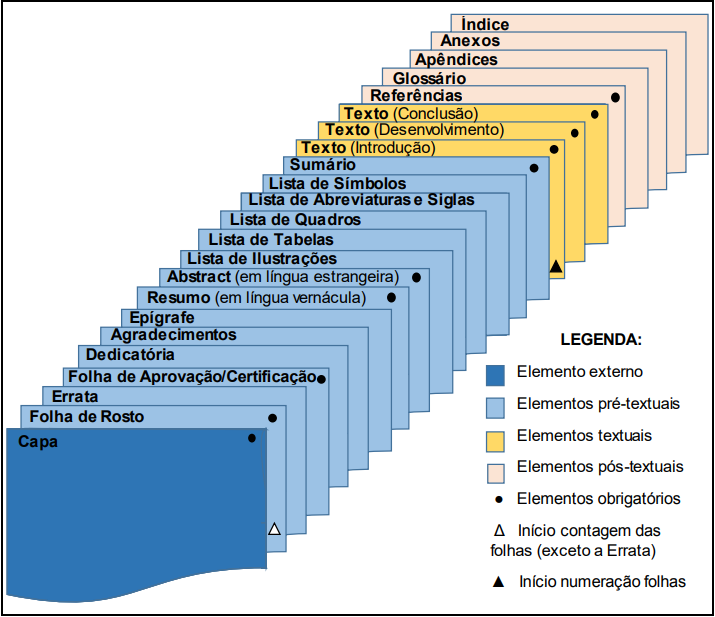
\includegraphics[width=10cm]{guia-elementos.png}
    
    \footnotesize
    Fonte: \textcite{livro:iffar-guia-normalizacao-2022}.
  \end{figure}

\section{Parte externa}
    \subsection{Capa (obrigatório)}
    Arquivo: \texttt{elementos/capa.tex}

    Não é computada na contagem das folhas.

    É configurado automaticamente pelo arquivo \texttt{elementos/DADOS.tex}. Selecione se o seu trabalho é TCC ou Tese e Dissertação e preencha os dados restantes com os valores necessários.

    O Guia de Normalização estabelece que a capa deve conter \blockcquote[p. 30]{livro:iffar-guia-normalizacao-2022}{nome da instituição (opcional), título do trabalho e nome do(a) autor(a)}, o mesmo estabelecido pela NBR 14724 \cite{livro:abnt-nbr:14724}, porém, nos seus exemplos visuais mostram-se dados adicionais\footnote{Eu implementei conforme o ilustrado, apesar de não saber sobre a definição de margens.}.

    \subsection{Lombada (opcional)}
    É utilizado para trabalhos impressos e, por isso, este modelo não abrange tal elemento.

\section{Elementos pré-textuais}
    Para o caso do uso da configuração \textbf{twoside}, para uso de verso e anverso das folhas: recomenda-se que seus elementos, com exceção da ficha catalográfica/de identificação, iniciem no anverso das folhas (parte da frente da folha, página ímpar). O modelo detecta e realiza a configuração para o início desses elementos\footnote{Porém, podem acontecer \textit{bugs}, pois o \texttt{cleardoublepage} é considerado um comando frágil pelo \LaTeX{}.}, você pode optar por desativar, comentando ou removendo os comandos \verb|\OnesideTwoside| no fim de cada elemento, apesar da utilização de pelo menos um \verb|\clearpage| ser recomendada\footnote{Mas também não acontece nenhum problema se não existir o comando}.

\subsection{Folha de rosto (obrigatório)}
    Arquivo: \texttt{elementos/folha-rosto.tex}

    Também configurado automaticamente pelo arquivo \texttt{elementos/DADOS.tex}. Caso a lógica criada para o preenchimento dos dados não funcione bem para a sua situação, não tenha receio em alterar diretamente o seu texto em seu arquivo.

    Para o caso do trabalho estar configurado como \textbf{twoside}, para a impressão no verso e anverso, configure, no final de seu arquivo, o uso do \verb|\clearpage|:
    \begin{alinea}
        \item se existir a ficha catalográfica\footnote{Que nem ao menos sei como que é realizado o processo, se o autor que adiciona no documento \LaTeX{} ou se o(a) bibliotecário(a) é responsável tanto por criar os dados quanto anexar depois no documento.}/identificação de obra, altere o comando \verb|\OnesideTwoside| e utilize \verb|\clearpage|, pois a ficha deve estar no verso;
        \item se ainda não possuir a ficha, seja qual for, deixe o comando \verb|\OnesideTwoside| decidir pelo \verb|\cleardoublepage|.
    \end{alinea}

\subsection{Ficha catalográfica ou ficha de identificação (obrigatório)}
    Arquivo: \texttt{elementos/ficha-catalografica.tex}

    A ficha catalográfica é elaborada pelos bibliotecários da instituição e a ficha de identificação é produzida pelos autores dos trabalhos, \blockcquote[p. 15]{livro:iffar-guia-normalizacao-2022}{partir de um sistema gerador que a instituição utilize}\footnote{Não tenho ideia alguma sobre esse sistema.}.

    Obrigatoriamente deve estar contida no verso da folha de rosto\footnote{Até mesmo utilizando \textbf{oneside}? Se for, acho que será necessário criar uma lógica diferente, pois assim não sei como que fica a contagem de páginas para este elemento.}.
    
\subsection{Errata (opcional)}
    Ocorre após a impressão do trabalho e, por isso, o modelo não abrange tal elemento. Se necessário, pode-se utilizar outra ferramenta de texto para gerar a errata, visto que só deve ser necessário manter a mesma fonte utilizada no trabalho.
    
\subsection{Folha de aprovação e/ou folha de certificação (obrigatório)}
    Arquivo: \texttt{elementos/folha-aprovacao.tex}

    Configurada automaticamente pelo arquivo \texttt{elementos/DADOS.tex}: para TCC é utilizada a folha de aprovação; e, para o caso de Tese ou Dissertação, utiliza-se a folha de certificação. Adicione seus dados e, se a lógica criada para o preenchimento dos dados não funcionar para o seu caso, não tenha receio de alterar manualmente o texto em seu arquivo.
    
\subsection{Dedicatória (opcional)}
    Arquivo: \texttt{elementos/dedicatoria.tex}

    Não possui título e a \blockcquote[p. 32]{livro:iffar-guia-normalizacao-2022}{a autoria de terceiros deve ser citada, e também deve constar nas Referências)}.

    Em \texttt{main.tex}, comente a linha \verb|\vspace*{\fill}

% Tamanho total da página: 21cm
% Margem esquerda: 3cm
% Margem direita: 2cm
% Recuo necessário: 4cm
% Espaço restante: 12cm
\hspace{\fill}
\begin{minipage}{12cm}
    \setlength{\parindent}{1.25cm}
    
    Este trabalho é dedicado [especificar o texto da dedicatória, escrito pelo(a) autor(a), registrando a quem dedica o Trabalho Acadêmico-Científico realizado ou prestando uma homenagem a alguém que considere importante no transcorrer do seu processo formativo (pessoal e/ou acadêmico-profissional), ainda que essa pessoa não tenha contribuído diretamente para os resultados obtidos no trabalho].
\end{minipage}

% Recomendação do Guia de Normalização de iniciar cada elemento pré-textual e textual no anverso da página
\OnesideTwoside{\clearpage}{\cleardoublepage}
| para não adicionar o elemento.

\subsection{Agradecimentos (opcional)}
    Arquivo: \texttt{elementos/agradecimentos.tex}

    \blockcquote[p.32]{livro:iffar-guia-normalizacao-2022}{Pode se constituir de um texto mais extenso, em que são mencionadas as contribuições relevantes para os resultados apresentados no trabalho.

    Sugere-se incluir a agência financiadora, indicando-se a fonte de
    financiamento que viabilizou a realização do estudo.}

    Em \texttt{main.tex}, comente a linha \verb|\chapter*{Agradecimentos}
\thispagestyle{empty}

\lipsum[2]| para não adicionar o elemento.

\subsection{Epígrafe (opcional)}
    Arquivo: \texttt{elementos/epigrafe.tex}

    Além de utilizar como elemento pré-textual, a epígrafe também pode ser utilizada para iniciar as seções primárias (capítulos) do seu trabalho, porém, é algo opcional. Para se criar uma epígrafe, utiliza-se de seu respectivo ambiente criado para este modelo, através do comando \verb|\begin{epigrafe}|.

    Nas epígrafes é recomendado o destaque em itálico para a citação e de negrito para a autoria dessa citação, que deve seguir o padrão para referenciamento, como sobrenome em caixa alta, ano e página envoltos entre parênteses, de acordo com o exemplo em \textcite[figura 14, p. 39]{livro:iffar-guia-normalizacao-2022}.

    Em \texttt{main.tex}, comente a linha \verb|\vspace*{\fill}

% Largura da folha: 21cm
% Margem à esquerda: 3cm
% Margem à direita: 2cm
% Espaço para texto: 16cm;
% Margem à esquerda necessária: 10cm
% Se for margem de 10cm da página inteira, tamanho de: 11cm
% Se for margem de 10cm da parte de texto, sem considerar os 3cm: 6cm 
\hspace{\fill}
\begin{minipage}{6cm}
    \begin{singlespace} % A epígrafe tem que usar espaçamento símples
        % Seu texto recomenda-se em itálico e autor em negrito
        \textit{Lorem ipsum dolor sit amet, consectetur adipiscing elit. Curabitur et neque metus. Ut volutpat sem quis lacus rutrum, a viverra odio tincidunt. Quisque eu mollis enim. Suspendisse porta vehicula pharetra. Sed magna risus, consequat vitae tempus at, pulvinar ut sapien. Donec sit amet metus feugiat massa molestie venenatis id vel est. Fusce dapibus nisi vitae urna suscipit, non hendrerit mauris consequat. Nunc in quam vel dolor auctor interdum eget nec metus. Donec ornare libero euismod mi vehicula tincidunt. Pellentesque fermentum vulputate lacus, sit amet facilisis dolor faucibus et} (\textbf{Autor}).
    \end{singlespace}
\end{minipage}

% Recomendação do Guia de Normalização de iniciar cada elemento pré-textual e textual no anverso da página
\OnesideTwoside{\clearpage}{\cleardoublepage}| para não adicionar o elemento.

\subsection{Resumo na língua vernácula (obrigatório)}\index{Elementos obrigatorios@Elementos obrigatórios!Resumo!na lingua vernacula@na língua vernácula}
    Arquivo: \texttt{elementos/resumo.tex}

    O resumo em língua portuguesa. Não é necessário configurar nada, apenas realizar a escrita\footnote{Que, inclusive, gostaria de recomendar o material desenvolvido por \textcite{pdf:resumo-aluisio}, caso você tenha dúvidas sobre como escrever um resumo.}.

\subsection{Resumo em língua estrangeira (obrigatório)}
    Arquivo: \texttt{elementos/abstract.tex}

    A presença deste elemento é obrigatória e o modelo traz seu exemplo para a língua inglesa, \textit{abstract}, porém, o resumo pode ser realizado em qualquer outro idioma de divulgação internacional\footnote{Recomendo a utilização do tradutor Deepl (\url{https://deepl.com/}) como ferramenta de apoio, se considerar necessário.}, apenas necessitanto editar seu arquivo, como o título traduzido para seu devido idioma.

\subsection{Lista de ilustrações (opcional)}
    Arquivo: \texttt{main.tex}

    O Guia de Normalização \cite{livro:iffar-guia-normalizacao-2022} estabelece a utilização de lista de ilustrações\footnote{Eu sempre fico medidor confuso com a distinção de lista de ilustrações e lista de figuras. São o mesmo?}, recomendando-se a criação de listas distintas para cada tipo, caso haja mais de cinco elementos do tipo, (figuras, quadros, gráficos, desenhos, fotografias, organogramas, gravuras e outros). No arquivo \texttt{main.tex}, algumas linhas abaixo de \verb|\usepackage{newfloat}|, estão contidas as instruções para a criação de outros elementos e suas listas.

    Em \texttt{main.tex}, comente as linhas das listas, como \verb|\listoffigures|, \\\verb|\listofquadros|, \verb|\listofgraficos|, etc., para não adicionar os elementos.

\subsection{Lista de tabelas (opcional)}
    Arquivo: \texttt{main.tex}

    Em \texttt{main.tex}, comente a linha \verb|\listoftables| para não adicionar o elemento.

\subsection{Lista de quadros (opcional)}
    Arquivo: \texttt{main.tex}

    Apesar de ser definido como elemento de ilustração, sua lista, de acordo com o Guia de Normalização, na Figura \ref{figura:elementos-guia}, é apresentada depois da lista de tabelas, que não é citada como exemplo de elemento de ilustração. Não foi identificado no Guia de Normalização a ordem de apresentação caso houvesse a criação de outras listas.

    Em \texttt{main.tex}, comente a linha \verb|\listofquadros| para não adicionar o elemento.

\subsection{Lista de abreviaturas e siglas (opcional)}
    Arquivo: \texttt{elementos/lista-siglas.tex}

    A ordenação de abreviaturas e siglas deve ser realizada alfabeticamente, manualmente pelo usuário, contudo, na primeira vez citada no texto, a sigla ou abreviatura deve ser apresentada entre parênteses precedido pela sua designação. E, para adicionar uma sigla à lista, no arquivo \texttt{elementos/lista-siglas.tex} utiliza-se o comando \verb|\sigla|.

    O espaçamento utilizado de margem para o alinhamento da sigla e seu significado pode ser alterado modificando a unidade de medida do comando \verb|\siglaLargura|

    Em \texttt{main.tex}, comente a linha \verb|% Crio um elemento utilizado para listar cada abreviatura e sigla
% Obs.: Dependendo do tamanho das siglas utilizadas, você pode querer aumentar ou diminuir o espaço entre a sigla e o seu significado, porém, mantendo o alinhamento, para isto, você modifica o comando \newcommand\siglaLargura{10ex}, substituindo o 10ex pelo tamanho que você deseja
% O tamanho 10ex suporta uma sigla de até mais ou menos 10 letras, visto que a unidade utiliza como referência o tamanho da letra "x". Você também pode utilizar a unidade "em", que utiliza como referência a letra "m", se quiser.
% Fonte: https://tex.stackexchange.com/a/508154
\newcommand\siglaLargura{10ex} % Comprimento do espaço onde fica a sigla
\newcommand\siglaGap{1ex} % Comprimento do vão entre sigla e seu significado, para dar uma folguinha no tamanho máximo
\newcommand\nomeSiglaLargura{\dimexpr\linewidth-\siglaLargura-\siglaGap\relax}
\newcommand\sigla[2]{\noindent\parbox[t]{\siglaLargura}{#1\strut}%
  \hspace{\siglaGap}%
  \parbox[t]{\nomeSiglaLargura}{#2\strut}}

% Adicione as suas siglas:
\chapter*{Lista de abreviaturas e siglas}
% Para adicionar uma abreviatura ou sigla na lista apenas precisa adicionar a sigla dentro do \sigla{<insira a sigla>}{<insira o nome completo da sigla>}

\sigla{IBGE}{Instituto Brasileiro de Geografia e Estatística}

\sigla{IFFar}{Instituto Federal de Educação, Ciência e Tecnologia Farroupilha}

\sigla{TCC}{Trabalho de Conclusão de Curso}

\sigla{T}{Teste}

\sigla{xxxxxxxxxx}{Lorem ipsum dolor sit amet, consectetur adipiscing elit. Curabitur et neque metus. Ut volutpat sem quis lacus rutrum, a viverra odio tincidunt}| para não adicionar o elemento.

\subsection{Lista de símbolos (opcional)}
    Arquivo: \texttt{elementos/lista-simbolos.tex}

    Os símbolos adicionados à lista devem ser inseridos conforme a ordem em que aparecem no texto e, na lista, \blockcquote[p. 32]{livro:iffar-guia-normalizacao-2022}{recomenda-se o uso das unidades de medida, após a descrição do símbolo, colocadas entre parênteses, quando for o caso}. Um símbolo é adicionado à lista através do comando \verb|\simbolo|, no arquivo \texttt{elementos/lista-simbolos.tex}.

    O espaçamento utilizado para o alinhamento do símbolo e sua descrição pode ser alterado modificando a unidade de medida do comando \verb|\simboloLargura|.

    Em \texttt{main.tex}, comente a linha \verb|% Crio um elemento utilizado para listar cada símbolo e seu significado
% Obs.: É a mesma lógica da lista de siglas. Ajuste o tamanho do comprimento da "caixinha" do símbolo conforme a sua necessidade
% Fonte: https://tex.stackexchange.com/a/508154
\newcommand\simboloLargura{5ex} % Comprimento do espaço onde fica o símbolo
\newcommand\simboloGap{1ex} % Comprimento do vão entre símbolo e seu nome, para dar uma folguinha no tamanho máximo
\newcommand\simboloNomeLargura{\dimexpr\linewidth-\simboloLargura-\simboloGap\relax}
\newcommand\simbolo[2]{\noindent\parbox[t]{\simboloLargura}{#1\strut}%
  \hspace{\simboloGap}%
  \parbox[t]{\simboloNomeLargura}{#2\strut}}

% Adicione os seus símbolos:
\chapter*{Lista de símbolos}

% Para adicionar uma abreviatura ou sigla na lista apenas precisa adicionar o símbolo no comando \simbolo{<insira o símbolo>}{<insira o significado do símbolo>}

\simbolo{\LaTeX}{LaTeX}

\simbolo{\S}{Parágrafo}

\simbolo{$\Sigma$}{Somatória}

\simbolo{$\sum_{n = 1}^{\infty}$}{Matemágica}

\simbolo{xxxxx}{Lorem ipsum dolor sit amet, consectetur adipiscing elit. Curabitur et neque metus. Ut volutpat sem quis lacus rutrum, a viverra odio tincidunt}

% Recomendação do Guia de Normalização de iniciar cada elemento pré-textual e textual no anverso da página
\OnesideTwoside{\clearpage}{\cleardoublepage}| para não adicionar o elemento.
    
\subsection{Sumário (obrigatório)}
    Arquivo: \texttt{main.tex}

    O espaçamento utilizado para o alinhamento do número da seção e seu título pode ser alterado modificando a unidade de medida do comando \verb|\espacoAlinhamentoSumario|.
    

\section{Elementos textuais}
    A parte textual dos trabalhos acadêmicos, o Guia de Normalização do IFFar estabelece a obrigatoriedade da apresentação de três elementos:
        \begin{alinea}
            \item introdução;
            \item desenvolvimento;
            \item e conclusão.
        \end{alinea}
    Essa é a definição lógica do que o conteúdo deve abranger e a ordem que deve ser apresentada, porém, não é a definição dos capítulos que a pessoa deve apresentar. Isso significa que a pessoa deve seguir essa estrutura lógica no seu conteúdo, mas tem total liberdade para definir os seus capítulos. Cada um desses três elementos possui suas particularidades e elas são mais detalhadas no Guia de Normalização.

    Para facilitar para quem está com dúvida, e essa é uma recomendação apenas do autor deste modelo, uma estrutura de capítulos seguida pode ser, por exemplo, e apenas se quiser\footnote{Cada área pode ter suas particularidades e também recomenda-se conversar com que lhe orienta para discutir como deve ser estruturado o seu trabalho}: 
        \begin{alinea}
            \item Introdução;
            \item Fundamentação teórica (ou Revisão da literatura);
            \item Metodologia;
            \item Análise e discussão dos resultados;
            \item Considerações finais (ou Conclusões).
        \end{alinea}

\section{Elementos pós-textuais}

\subsection{Referências (obrigatório)}
    As referências bibliográficas utilizadas no trabalho devem ser registradas no arquivo \texttt{bibliografia.bib}, ou outro arquivo de mesma extensão que for adicionado. Cada registro precisa seguir o modelo dos registros do \texttt{biblatex}, que se baseia no \texttt{bibtex} e, para auxiliar os mais inexperientes, encontram-se documentos na pasta \texttt{docs/} deste modelo, além do capítulo \ref{capitulo:referencias}, onde o tema é aprofundado.

\subsection{Glossário (opcional)}
    Arquivo: \texttt{elementos/glossario.tex}
    
    \blockcquote[p. 33]{livro:iffar-guia-normalizacao-2022}{Trata-se de uma relação de palavras ou expressões técnicas utilizadas no texto, de uso restrito ou de múltiplos sentidos, acompanhadas das respectivas definições. Os termos especificados são apresentados em ordem alfabética, seguidos de dois pontos, de um espaço e da
    explicação.}

\subsection{Apêndices (opcional)}\index{Apendice@Apêndice|see{Elementos opcionais}}
    Arquivo: \texttt{main.tex}
    
    Apêndices são elementos, como documentos e outros materiais, elaborados pelo próprio autor do trabalho. Eles devem ser adicionados dentro do ambiente \texttt{SecoesNaoNumeradas}, após as referências bibliográficas, e são criados através do comando \verb|\apendice|, que funciona exatamente como um capítulo, porém, com as adaptações exigidas pelo Guia de Normalização.

    Se o usuário quiser, pode criar um arquivo \texttt{.tex}, exatamente como os capítulos, e importá-los no arquivo principal, para manter o arquivo principal mais organizado.

\subsection{Anexos (opcional)}
    Arquivo: \texttt{main.tex}
    
    Anexos, diferentemente dos apêndices, são documentos elaborados por terceiros, utilizados pelos autores para complementar seus trabalhos. Apresentam a mesma lógica dos apêndices para a utilização no modelo, contudo, usando o comando \verb|\anexo| para criar a seção específica do anexo. A mesma recomendação sobre criar um arquivo específico para apêndice é válida para os anexos, melhorando a organização do trabalho.

\subsection{Índice (opcional)}\index{Indice@Índice|seealso{Elementos opcionais}}
    Arquivo: \texttt{main.tex}

    O índice é utilizado para apresentar onde determinados termos e temas são abordados em um trabalho. Podem ser utilizados diversos elementos para apresentar a localização, como página, seção, elementos como anexos, contudo, existem algumas limitações do que pôde ser implementado para este modelo.
    
    Para a implementação do índice foi utilizado o pacote \texttt{imakeidx}, e ele apresenta limitações em alguns aspectos. A primeira limitação no modelo é que o índice possui a capacidade de apenas poder apresentar a página de onde encontra-se o termo, não sendo possível, de forma prática, apresentar seções ou outros elementos. Um segunda limitação é a de que o \texttt{imakeidx} não sabe lidar com caracteres especiais, como caracteres acentuados, ou também de outros idiomas além do padrão Latin XXXXX, para realizar o ordenamento alfabético. Isso significa que quando o termo possuir uma letra acentuada, por exemplo, é necessário utilizar o comando de uma forma alternativa. Além dessas limitações do pacote, também houve a implementação apenas para a apresentação do índice por ordem alfabética. Outras formas de índice, estabelecidas pela NBR 6034, como ordem sistemática, ou cronológica, e de enfoque especial, ficam a critério de serem implementadas pelo usuário\footnote{E nem sei o quão prático seria implementar, pois, acredito que seria necessário ter que utilizar outro pacote ou tecnologia para gerar o índice (o \texttt{imakeidx} suporta algumas outras para gerar e formatar índices)}.

--- Índice\\
    - Mostrar como usar os comandos, alertando que ele não imprime na tela a palavra
    - Mostrar as palavras ``nested''

    Testar se consegue ter mais de 3 níveis de itens
    Falar que implementou apenas a forma alfabética de índice, fica por conta da pessoa formatar para outras formas
    Testar range de páginas (--)
    Falar dos caracteres acentuados (e de outros idiomas, se o usuário for tentar)
    Falar da limitação de apenas apresentar o número de página
    Falar de cabeçalho simples (1 só) e cabeçalho composto (nested)
    Remissivas (duplicar para o caso de ver também)
        Limitação da remissiva ver também (quebrar a linha e repetir o item )
    Recomendar criar comandos para imprimir sempre as mesmas entradas
        Criar no início dos capítulos, ou no início do documento, ou criar um arquivo específico para entradas no índice
        É muito fácil se confundir e digitar uma letrinha diferente, com um espaço diferente, principalmente se tiver caracteres acentuados
    Se quiser, utilizar um comando que tanto cria o índice quanto escreve na tela
    Use apenas 1 ver também ou ver por termo

    % \index{<palavra para ordenar>!<palavra impressa>}

    \iindex{Carlos} Teste
    
    \index{Carlosa@Carlos|seealso{Rogério}}
    
    \indexsee{Carlos}{Glauber}{}{}Teste2
    
    \indexsee{Índice}{Glauber}{Perere!}{Indice}Teste2
    
    \indexseealso{Carlos}{Mané}{}{}Teste3

    \ifEmpty{Não}{Não vazio}{Vazioo}
    
  % Recomendação do Guia de Normalização de iniciar cada elemento pré-textual e textual no anverso da página
  \OnesideTwoside{\clearpage}{\cleardoublepage}
\endgroup

\begingroup
  \chapter{Exemplos de elementos comuns} % Exemplo de seção primária
  Neste capítulo é apresentado um conjunto de elementos comuns que provavelmente serão utilizados em algum momento por todos os autores de trabalhos acadêmicos, como figuras e tabelas. Por questão de praticidade, no texto, não será discutido o código que leva à impressão de determinado elemento, talvez com algumas pequenas exceções. O objetivo deste capítulo é apresentar seus exemplos, realizando algumas observações sobre cada elemento, porém, tendo no código do capítulo, no arquivo \verb|capitulos/4-elementos-comuns.tex|, a exemplificação de como utilizar determinado elemento no \LaTeX, com comentários, para maiores explicações.

  \section{Exemplos de seções} % Exemplo de seção secundária
  Essa aqui é um exemplo de seção secundária, mas as seções, ao todo, podem apresentar até 5 (cinco) níveis de subdivisão. A seção primária, como pode ter sido observado, são os capítulos, mas, a seguir, apresentam-se as outras seções.

  \subsection{Exemplo de seção terciária}
  \lipsum[1]

  \subsubsection{Exemplo de seção quaternária}
  \lipsum[2]

  \paragraph{Exemplo de seção quinária} % Utiliza-se paragraph para o nível hierarquico inferior à subsubsection. Contudo, foi necessário customizá-lo para apresentar corretamente como um nível de seção
  \lipsum[3]

  \paragraph{Exemplo de título com indicação numérica que, ao ocupar mais de uma linha, deve ser, a partir da segunda linha, alinhado abaixo da primeira letra da primeira palavra do título}
  \lipsum[4]

\section{Notas de rodapé}
  As notas de rodapé devem apresentar tamanho 10, alinhamento à esquerda e espaçamento justificado, além de, ao utilizar mais de uma linha, deve ser alinhado abaixo da primeira letra da primeira palavra da primeira linha\footnote{\lipsum*[5]}. No \LaTeX{} existe um conjunto de comandos para utilizá-las, por exemplo, a nota pode ser adicionada no meio do parágrafo\footnote{Exatamente como a primeira nota}, porém, também pode ter apenas a sua marcação realizada no parágrafo\footnotemark, permitindo preencher o seu texto posteriormente.
    \footnotetext{Exemplo de nota usando a marcação.}
  
  É importante relatar que existe um problema ao utilizar apenas a marcação: o comando para adicionar o texto à nota utiliza apenas o número da nota de rodapé mais recente\footnotemark, então, se você adicionar duas \verb|\footnotemark| seguidas\footnotemark, deixando os dois \verb|\footnotetext| para depois, será utilizada apenas o número da última nota criada, com as duas notas apresentando o mesmo número. 
    \footnotetext{Nota relativa à primeira marcação.}
    \footnotetext{Nota relativa à segunda marcação.}
  Dessa forma, a recomendação é utilizar o \verb|\footnotemark| apenas quando o parágrafo possuir apenas uma nota ou adicionar o texto da marcação após o término da frase e não do parágrafo. Ou, então, não utilizar, realizando a quebra de linha se quiser deixar mais formatadinho o código no \LaTeX\footnote{Um novo parágrafo só é criado quando existirem duas quebras de linhas seguidas, ou seja, uma linha em branco.}.

\section{Alíneas e subalíneas}
  As alíneas\index{alíneas} sempre devem vir a partir de um parágrafo que termine com dois pontos antes de iniciar a lista:
  \begin{alinea}
    \item a matéria da alínea começa por letra minúscula, exceto quando se tratar de substantivos próprios, e termina em ponto e vírgula, com exceção da última, que termina em ponto final;
    \item o trecho final da seção correspondente, anterior às alíneas, termina em
    dois pontos;
    \item as alíneas são ordenadas por letras minúsculas seguidas de parênteses utilizando-se letras dobradas quando esgotadas as 26 (vinte e seis) letras que compõem o alfabeto brasileiro;\label{alinea:exemplo-ref}
    \item as letras indicativas das alíneas são recuadas em relação à margem
    esquerda, alinhadas com o parágrafo;
    \item o texto da alínea deve terminar em dois pontos, se houver subalíneas\index{subalíneas}: 
    \begin{subalinea}
      \item a matéria da subalínea começa por letra minúscula e termina em ponto e
      vírgula, e a última subalínea deve terminar em ponto final, se não houver
      alínea subsequente; 
      \item são iniciadas por travessão seguido de espaço;
      \item devem apresentar recuo em relação à alínea;
      \item a segunda linha e as demais que se seguem no texto da subalínea
      começam sob a primeira letra do texto da própria subalínea.
    \end{subalinea}
    \item a segunda linha e as demais que se seguem no texto da alínea começam
    sob a primeira letra do texto da própria alínea.
  \end{alinea}
E se você não quebrar a linha para iniciar um novo parágrafo, o \LaTeX{} continuará no mesmo parágrafo, não realizando a indentação, contudo, eu não sei se isso é algo desejado. Eu não encontrei nenhuma norma na ABNT que falasse sobre isso, nem algum exemplo no Guia de Normalização. Na dúvida, é só quebrar a linha duas vezes, para começar um novo parágrafo

  % \subsection{Outros exemplos de listas numeradas}
    % \begin{leiParagrafo}
    %   \item a matéria da alínea começa por letra minúscula, exceto quando se tratar de     substantivos próprios, e termina em ponto e vírgula, com exceção da última, que termina em ponto final; 
    %   \item o trecho final da seção correspondente, anterior às alíneas, termina em
    %   dois pontos;
    %   \item asdasdsada
    %   \item sdsdsdaa
    % \end{leiParagrafo}

\section{Equações e fórmulas}
  Existe um grande número de pacotes para a impressão de elementos e símbolos matemáticos\footnote{Vou ser bem honesto, isso aqui não é nem um pouco a minha área. Estou citando aqui por causa que é um ponto importante, mas não tenho ideia direito do que estou falando.}. Este modelo, por exemplo, já tem importado o pacote \texttt{amssymb}, para a adição de símbolos, e o \texttt{amsmath}\footnote{Adicionei só para ajudar quem não conhece sobre, se você não utilizar nada ``matemático demais'', esse pacote pode ser tranquilamente removido.}, para maiores funcionalidade com elementos matemáticos, mas nada impede a adição de outros pacotes. Porém, deve-se atentar com o  conflito de pacotes. Dependendo do que os pacotes fazem, principalmente se tiverem funcionalidades muito semelhantes, pode ocorrer conflito, levando a erros na compilação. E isto é uma recomendação geral sobre pacotes. Não é necessário ter receio de adicionar outros pacotes, porém, eles devem ser adicionados com atenção, visualizando quais pacotes o modelo já utiliza.

  Para a apresentação de expressões matemáticas, o \LaTeX{} apresenta muitas maneiras para se utilizar, podendo ocorrer de dois modos: \textit{inline} e \textit{display}. O primeiro é para expressões que fazem parte de um parágrafo e o segundo é utilizado em um bloco de texto exclusivo para a expressão. Seguem-se exemplos:

  No modo \textit{inline} pode ser escrito expressões de várias formas, como: \(E=mc^2\); $ 2 \times 2 = 4 $; e, também, \begin{math} x^2 + y^2 = z^2 \end{math}. Contudo, o Guia de Normalização estabelece que equações e fórmulas devem aparecer \blockcquote[p. 23]{livro:iffar-guia-normalizacao-2022}{destacadas no texto, a fim de facilitar sua leitura}.
  
  E, para o modo \textit{display}, também existem múltiplas formas de adicionar uma expressão ao texto:
  \[ x^n + y^n = z^n \]
  
  Ou:
  \begin{displaymath}
    \sqrt{x^2+1}
  \end{displaymath}
  
  Ou, então:
  \begin{equation}
    e^{\pi i} + 1 = 0
  \end{equation}

  Também existe o ambiente \texttt{equation*}, provido pelo pacote \texttt{amsmath}\footnote{Esse exemplo foi extraído do pacote, para mostrar as possibilidades. Recomendo demais a leitura (olhadinha rápida) da documentação do pacote, caso tenha interesse.}:
  \begin{equation*}
    \left.\begin{aligned}
    B’&=-\partial\times E,\\
    E’&=\partial\times B - 4\pi j,
    \end{aligned}
    \right\}
    \qquad \text{Maxwell’s equations}
  \end{equation*}

  O \texttt{amsmath} também provê um grande número de funcionalidades, para realizar o alinhamento das expressões\footnote{Recomendação de leitura: \url{https://www.overleaf.com/learn/latex/Aligning_equations_with_amsmath}}:
  
  \begin{equation}
    \begin{split}
      A& = \frac{\pi r^2}{2} \\
       & = \frac{1}{2} \pi r^2
    \end{split}
  \end{equation}
  
  Ou:
  \begin{multline}
    p(x) = 3x^6 + 14x^5y + 590x^4y^2 + 19x^3y^3\\ 
    - 12x^2y^4 - 12xy^5 + 2y^6 - a^3b^3
  \end{multline}

  A ABNT prevê também, e de maneira opcional, a possibilidade de realizar a numeração das equações. Como é observável, o próprio elemento \texttt{equation} do \LaTeX{} já apresenta sua própria numeração, além de alguns outros elementos do \texttt{amsmath} porém, também existem maneiras de desativar essa função\footnote{Posso ter entendido errado, mas o equation* do \texttt{amsmath} tem a exata diferença de não ter numeração.}.

\section{Figuras, tabelas e quadros}
  Sobre elementos como as figuras\index{figura}, tabelas\index{tabela} e quadros\index{quadro}, é importante destacar que o comando utilizado para criar esses elementos é apenas um invólucro, onde você pode colocar o conteúdo que quiser dentro deles. E esse invólucro é apenas responsável por dar o ``tratamento'' como determinado item, e aí, dentro dele, são realizados os comandos que realmente adicionam os itens pertinentes ao respectivo elemento, como uma imagem, no caso de figuras.
  
\subsection{Figuras}
  Para as figuras, podem ser utilizados os formatos de imagens mais populares, como \verb|.png| ou \verb|.jpg|\footnote{É válido pesquisar quais são todos os formatos aceitos}, porém, além de imagens, também podem ser adicionados documentos \verb|.pdf|. A vantagem de utilizar um \textit{Portable Document Format} (PDF) é que os textos contidos não perderão a qualidade, por não passarem por compressão, ao imprimir as palavras diretamente como texto, como ilustrado na Figura \ref{figura:pdf}. Porém, apesar de aceitar formatos populares de imagens, nativamente (e pelo pacote utilizado), imagens \textit{Scalable Vector Graphics} (SVG) não são possiveis de serem utilizadas. Inclusive, até existem pacotes que adicionam a capacidade de imprimir SVGs nos documentos, porém, eles possuem um conjunto de limitações\footnotemark. A seguir, na Figura \ref{figura:marca-iffar}, é apresentado um exemplo com a marca do IFFar.
      \footnotetext{Dependendo do programa que você estiver usando, você pode exportar a figura como PDF, logo, conseguindo imprimir corretamente a imagem, eu acho.}

  \begin{figure}[H]
    \Centering\singlespacing
    \caption{Marca do IFFar}
    \label{figura:marca-iffar} % Esse é o comando que permite referenciar a figura (ou qualquer outro elemento que você criar)
    % Podem ser utilizados vários argumentos para adicionar a figura em seu devido tamanho, como: scale; width; ou height. No caso de scale, a escala, adiciona o valor em decimal representando a porcentagem da escala, já width ou height utiliza-se uma unidade de medida, como cm, px ou pt.
    
\includegraphics[width=10cm]{marca-iffar.png}\\
    \footnotesize
    Fonte: \textcite{site:iffar-identidade-visual-2021}.
  \end{figure}

  \begin{figure}[H]
    \Centering\singlespacing
    \caption{Exemplo utilizando documento PDF}
    \label{figura:pdf}
    
\includegraphics[scale=1.0]{exemplo.pdf}\\
    \footnotesize
    Fonte: elaborado pelo autor (2023).
  \end{figure}
  
\subsection{Tabelas}
  Como citado anteriormente, os elementos das figuras, tabelas e quadros são apenas um invólucro, então, para tabelas (e quadros), podem ser utilizados um conjunto de alternativas para gerarem-se as tabelas. No caso deste modelo, pode ser utilizadas para gerar as tabelas as opções de \verb|tabular|, nativo do LaTeX, e \verb|tabularx|,adicionado através de um pacote e que permite criar tabelas com variados tamanhos de colunas. Existem também outros pacotes que permitam gerar tabelas e, então, pode ser útil pesquisar sobre eles. Na Tabela \ref{tabela:barbetta-2017-p248} é apresentada uma tabela utilizando \verb|tabular| e, na Tabela \ref{tabela:exemplo-caracteres}, utilizando \verb|tabularx|.

\begin{table}[H]
  \Centering\singlespacing

  \caption{Classificação de pessoas segundo o nível de instrução e colaboração
  com a coleta seletiva do lixo
  }
  \label{tabela:barbetta-2017-p248}
  \begin{tabular}{l|c|c} % As pipelines "|" indicam onde deve haver uma linha separando as células e as letras indicam o alinhamento do conteúdo das células da coluna
    \hline % Adiciona um traço horizontal na tabela
    \multirow{2}{*}{Nível de instrução} & \multicolumn{2}{c}{Colabora com a coleta seletiva do lixo} \\ % Por causa do \multicolumn, essa linha não apresenta o último "&" para a última célula e o "\\" finaliza a linha
    \cline{2-3} % Já que o \hline nessa linha iria desconfigurar por causa do \multirow, é necessário criar uma linha que inicie de determinada coluna e termine em outra coluna determinada
    & \parbox{3cm}{\Centering sim} & \parbox{3cm}{\Centering não} \\  % Por conta do \multirow na linha acima, a primeira célula dessa linha fica em branco
    \hline
    nenhum ou fundamental & 22 & 13 \\
    médio & 33 & 34 \\
    superior & 39 & 36\\
    \hline
   \end{tabular}

\hspace{\fill}

\footnotesize

Fonte: \textcite[p. 248]{livro:barbetta-2017}.
\end{table}

\begin{table}[H]
  \Centering\singlespacing

  \caption{Exemplos de caracteres especiais no LaTeX}
  \label{tabela:exemplo-caracteres}

  \begin{tabularx}{0.65\textwidth} { 
    >{\centering\arraybackslash}X 
    | >{\centering\arraybackslash}X}
    \hline
    Comando    & Caractere   \\ \hline
    \verb|\&|  & \&          \\ \hline
    \verb|\$|  & \$          \\ \hline
    \verb|\{|  & \{          \\ \hline
    \verb|\}|  & \}          \\ \hline
    \verb|\_|  & \_          \\ \hline
    \verb|$\backslash$|  & $\backslash$          \\ \hline
    \verb|\#|  & \#          \\ \hline
    \verb|\textemdash|       & \textemdash        \\ \hline
    \verb|\textendash|       & \textendash        \\ \hline
    %\verb|\textbar|          & \textbar           \\ \hline
    n\verb|\textordmasculine{}|          & n\textordmasculine{}           \\ \hline
    \verb|\textordfeminine{}|          & \textordfeminine{}           \\ \hline
    \verb|\textregistered|   & \textregistered    \\ \hline
    \verb|\copyright|        & \copyright         \\
    \hline
  \end{tabularx}

  \hspace{\fill}

  % A quebra de linha é essencial para o espaço horizontal ser corramente ocupado, não ocorrendo do texto de fonte ficar posicionado na posição errada, não centralizada
  \footnotesize
  Fonte: elaborado pelo autor (2023).

  Nota: há a exceção, específica para este modelo, dos caracteres º e ª, pois eles foram definidos como símbolos \textit{unicode} aceitos, no arquivo \texttt{config/unicode-char.sty}. O mesmo pode ser realizado para alguns outros exemplos, se optado, como o \textregistered{} ou \copyright. Além disso, o --- e o -- também podem ser realizados através de 3 e 2 híphens seguidos, respectivamente.
\end{table}

\subsection{Quadros}
  Para apresentar um quadro, utiliza-se a mesma lógica das tabelas. Na verdade, as únicas coisas que diferenciam um quadro de uma tabela é o termo utilizado para criar o elemento, \verb|\begin{quadro}|, e o fato que quadros são todo cobertos por bordas, enquanto que tabelas não apresentam bordas nas extremidades laterais. E essa borda é impressa ao adicionar os \textit{pipelines} (``|'') nas extremidades, ao definir as colunas do \verb|tabular[x]| (ex.: \verb|\begin{tabular}{|\textbf{|}\verb\c|c|c\\textbf{|}\verb|}|). A seguir, no Quadro \ref{quadro:exemplo}, isso pode ser visualizado.

  \begin{quadro}[H]
    \Centering\singlespacing
  
    \caption{Exemplo de quadro com múltiplas linhas e colunas}
    \label{quadro:exemplo}
  
    \begin{tabularx}{0.65\textwidth}
      {|c|r|l|X|} % Definição das colunas
      \hline
      Coluna 1  & Coluna 2  & Coluna 3  & Coluna 4 \\
      \hline
      \multicolumn{2}{|c|}{Itens 1 e 2} & Item 3    & Item 4 \\
      \hline
      Item 5    & Item 6    & Item 7   & \multirow{2}{*}{Itens 8 e 12} \\
      \cline{1-3}
      \multirow{3}{*}{\begin{sideways}9,13,17\end{sideways}}& Item 10   & Item 11  &                                   \\
      \cline{2-4}
      & Item 14   & \multicolumn{2}{c|}{\multirow{2}{*}{Itens 15, 16, 19 e 20}} \\
      \cline{2-2}
      & Item 18  & \multicolumn{2}{c|}{}\\
      \hline
    \end{tabularx}
  
    \hspace{\fill}
  
    % A quebra de linha é essencial entre o \hspace e outras linhas
    \footnotesize
    Fonte: elaborado pelo autor (2022).
  \end{quadro}

  % Recomendação do Guia de Normalização de iniciar cada elemento pré-textual e textual no anverso da página
  \OnesideTwoside{\clearpage}{\cleardoublepage}
\endgroup

\begingroup
  \chapter{Citações e referências}
Uma das características mais positivas do \LaTeX{} é a capacidade de gerenciar o uso de referências e citações, que podem ser referenciações de elementos presentes em seu texto ou citações de referências bibliográficas. E, para referências bibliográficas\footnotemark, este modelo utiliza o pacote \verb|biblatex|, junto com a sua opção de formatação da ABNT. Então, este capítulo busca trazer um conjunto de exemplos do uso dessas referências, também levando em consideração o \verb|biblatex|, para formatar corretamente. O pacote não tem como possuir a formatação dos inúmeros tipos de documentos padronizados pela ABNT, sendo necessário, às vezes, dar uma adaptada para conseguir a formatação desejada.
  \footnotetext{Neste capítulo são apresentados exemplos de referências considerando especificamente o \LaTeX, contudo, se tiver maiores dúvidas referências, é essencial que você consulte o Guia de Normalização de trabalhos do IFFar ou a norma ABNT NBR 6023:2018. Os dois documentos trazem exemplos de referências, mas, principalmente, o Guia também traz um conjunto de exemplos de como as citações devem ser realizadas.}

\section{Referênciação de elementos do texto}\label{section:referencia}
Um aspecto básico, e muitas vezes necessário, é a referênciação de elementos presentes pelo seu texto, como figuras ou seções. O comando que permite criar essa referência é o comando \verb|\label|\footnote{\label{rodape:exemplo-ref}Uma dica é você criar um padrão nos nomes dos rótulos para facilitar a identificação e evitar o risco de repetir nomes, iniciando com o nome do tipo de elemento que você está querendo referenciar e depois o nome do elemento, utilizando dois pontos para separá-los, como \texttt{tabela:nome-tabela} ou \texttt{figura:nome-figura}.}, 
e, apesar de ser mais comum ver este comando presente em figuras ou tabelas, também serve para referenciar seções, notas de rodapé e outros elementos que possuam contadores, como as equações, apêndices ou outros elementos criados pelo usuário\footnote{Os elementos criados, como os próprios quadros foram, mas também outros que forem criados pelo usuário, por exemplo, o elemento de Gráfico, também funcionarão se configurados corretamente.}. 
Depois, a citação é realizada através do comando \verb|\ref|, porém, é importante citar de que o comando do rótulo apenas seleciona o número do elemento, necessitando escrever separadamente o nome do elemento citado, como, por exemplo, citando a nota de rodapé \ref{rodape:exemplo-ref}, a Figura \ref{figura:marca-iffar}, o Anexo \ref{anexo:teste} ou a seção \ref{section:referencia}\footnote{Nisso, a padronização dos nomes, citados na nota \ref{rodape:exemplo-ref}, facilita bastante a identificação do elemento quando citados, para não se confundir na escrita.}. %ou a alínea \ref{alinea:exemplo-ref}. % O \ref para alíneas faz vir com o ) no nome, então não é tão útil

\section{Referências bibliográficas}
O gerenciamento das referências bibliográficas é realizado através do \verb|biblatex|, e o mesmo apresenta um conjunto de funções que podem ser utilizadas para facilitar a escrita. A primeira, e bastante importante, é que as obras da seção de referências só serão impressas se invocadas ao menos uma vez no documento através de citação. E, para as citações, existe um grande conjunto de comandos para citar as obras\footnote{\label{nota:biblatex-cheatsheet}No arquivo \texttt{docs/biblatex.pdfXXXXXXXX} encontra-se a documentação de um conjunto de comandos e registros utilizados pelo \texttt{biblatex}. Utilize-o como uma referência, para quando não souber os campos a serem utilizados no registro da referência ou os comandos para citações. Este capítulo do modelo busca apenas trazer uma ideia geral, não documentar tudo.}.

\subsection{Tipos e exemplos de citações}
\subsubsection{Citação indireta}
A citação indireta, que ocorre pela própria interpretação das palavras dos autores, pode ser realizada de duas formas: \verb|\cite| ou, para citar o autor diretamente no texto, \verb|\textcite|:

\verb|\cite{livro:dom-casmurro}|

\cite{livro:dom-casmurro}\\

\verb|\textcite{livro:dom-casmurro}|

\textcite{livro:dom-casmurro}

\paragraph{Citação simultânea de múltiplas obras}
Existem situações em que também é necessário citar simultaneamente mais de uma obra e, nesses casos, podem, também, ser realizadas de duas formas: \verb|\cites| ou, citando diretamente no texto, \verb|\textcites|:

\verb|\cites{site:iffar-identidade-visual-2021}{livro:dom-casmurro}|

\cites{site:iffar-identidade-visual-2021}{livro:dom-casmurro}\\

\verb|\textcites{site:iffar-identidade-visual-2021}{livro:dom-casmurro}|

\textcites{site:iffar-identidade-visual-2021}{livro:dom-casmurro}\\

Contudo, é importante citar que o \verb|biblatex| não realiza o ordenamento alfabético das múltiplas obras citadas, sendo função do autor do trabalho realizar esse controle na ordenação das entradas.

\subsubsection{Citação direta e citação direta longa}
Para citações de mais de três linhas, é necessário adicioná-las a um novo parágrafo, com 4cm de recuo, espaçamento simples e fonte tamanho 10, sem a presença de aspas. No \LaTeX, isso é alcançado através do comando \verb|\blockcquote|, do pacote \verb|csquotes|, que ajusta automaticamente para o formato de citação longa quando ultrapassa as três linhas. Porém, aqui existe um alerta: o comando utilizado recomendado é o \texttt{blockcquote} e não o comando \texttt{blockquote}, tendo, então, a letra \textbf{c} entre \texttt{block} e \texttt{quote}.

Os dois comandos, \verb|\blockcquote| e \verb|\blockquote|%
\footnote{Sendo justo, eu também não consegui fazer o \texttt{blockquote} funcionar corretamente com as citações do \texttt{biblatex}. Por isso recomendo o uso do \texttt{blockcquote}, que além de funcionar certinho, permite adicionar as informações anteriores e posteriores à obra citada.} 
apresentam a mesma funcionalidade. Contudo, o \verb|\blockcquote| apresenta três argumentos para citações, permitindo adicionar informações adicionais anteriores e posteriores à fonte, como o número de páginas da citação direta, exigido pela ABNT. A grande vantagem de utilizar esse comando, é que ele cria o ambiente de citação de forma automática, ou seja, se o texto inserido possuir até três linhas, a citação aparece entre aspas no corpo do parágrafo, mas se apresentar mais de três linhas, é ajustado como o parágrafo com recuo e as outras formatações necessárias.

Por conta da característica do comando de se ajustar automaticamente, a citação pode ser inserida no meio do parágrafo e, se ela tiver até três linhas, \blockcquote{batman}{aparece no mesmo parágrafo (você também pode apenas colocar o conteúdo entre aspas, `se quiser')}, porém, se possuir mais de três linhas, torna-se um parágrafo separado:
\blockcquote[tradução nossa]{filme:bee-movie}{De acordo com todas as leis conhecidas da aviação, não há como uma abelha poder voar. Suas asas são muito pequenas para tirar seu pequeno corpo gordo do chão. A abelha, obviamente, voa de qualquer maneira, porque abelhas não se importam com o que humanos pensam ser impossível}

\subsubsection{Citação apud}
O \texttt{biblatex-abnt} introduz um conjunto de comandos para citações apud, contudo, os comandos adicionam as duas fontes na bibliografia. Isso contradiz o estabelecido no Guia de Normalização, que indica que a fonte original, ao qual não se tem acesso, não é adicionada. Porém, esse problema é resolvido ao adicionar o campo \verb|keywords = {apud}| no registro da fonte original\footnote{Observe o registro do campo \texttt{keywords} do \texttt{exemplo:apud} no arquivo \texttt{bibliografia.bib}.}, já que a impressão da bibliografia foi configurada para filtrar os registros dessa maneira. Por exemplo, citando tem-se o resultado esperado, com a fonte original \texttt{exemplo:apud} não aparecendo na lista de referência.

Os comandos presentes para as citações apud são \verb|\apud| e \verb|\textapud|:

\verb|\apud[p. 79]{exemplo:apud}[p. 45]{batman}|

\apud[p. 79]{exemplo:apud}[p. 45]{batman}\\

\verb|\textapud{exemplo:apud}{batman}|

\textapud{exemplo:apud}{batman}\\

Também existem alternativas para caso não seja desejado ter o registro da fonte original no arquivo de bibliografia, \texttt{.bib}:

\verb|\apud[Um Autor Imaginário][]{batman}|

\apud[Um Autor Imaginário][]{batman}\\

\verb|Um Autor Imaginário \apud[apud][p. 42]{batman}|

Um Autor Imaginário \apud[apud][p. 42]{batman}

\subsubsection{Citação por outros elementos da referência}
Quando busca-se citar por alguns elementos diferentes da obra, como o título de uma obra, ou seu ano, podem ser utilizados determinados comandos para realizar tal função\footnotemark. Isso facilita o trabalho, por não precisar realizar a escrita manualmente, diminuindo as chances de erros, caso seja necessário atualizar algum dado da obra.
  \footnotetext{Como citado na nota \ref{nota:biblatex-cheatsheet}, o documento PDF traz um conjunto de comandos. Você pode consultá-lo para visualizar outros exemplos.}

Para citar pelo título da obra, utiliza-se \verb|\citetitle|, ou, que também possui outras utilidades, \verb|\citefield|, por exemplo: 

\verb|\citetitle{livro:dom-casmurro}| ou \\\verb|\citefield{livro:dom-casmurro}{title}|

\citetitle{livro:dom-casmurro} ou \citefield{livro:dom-casmurro}{title}\\

Para citar apenas o ano, \verb|\citeyear|, por exemplo: 

\verb|\citeyear{livro:dom-casmurro} ou \citeyear*{livro:dom-casmurro}|

\citeyear{livro:dom-casmurro} ou \citeyear*{livro:dom-casmurro}\\

Para citar apenas os nomes dos autores existem várias opções, a primeira é o \verb|\citeauthor|, por exemplo: 

\verb|\citeauthor{livro:dom-casmurro} ou \citeauthor*{livro:dom-casmurro}|\\

Também pode-se utilizar o \verb|\citename|, com um conjunto de configurações: 

\verb|\citename{livro:dom-casmurro}{author}| ou \\\verb|\citename{livro:dom-casmurro}[given-family]{author}|

\citename{livro:dom-casmurro}{author} ou \citename{livro:dom-casmurro}[given-family]{author}\\

Ou então utilizar o código criado para este modelo, \verb|\citeauthorfull|\footnotemark:
\footnotetext{Não garanto o pleno funcionamento deste comando em todas as situações. Eu realizei a adaptação de dois códigos distintos e, sendo bem honesto, não entendo bem exatamente como funciona a parte lógica do \texttt{biblatex}. Eu só vou experimentando até uma hora funcionar.}

\verb|\citeauthorfull{livro:dom-casmurro}|

\citeauthorfull{livro:dom-casmurro}\\

E também existe a opção de citar determinados campos dos registros das referências, como já mostrado anteriormente, através do comando \verb|\citefield|\footnote{Nem todos os campos funcionam, pois alguns são listas e, então, também apresenta comando específico para tal.}:

\verb|\citefield{lei:brasil-11.892-2008}{titleaddon}|

\citefield{lei:brasil-11.892-2008}{titleaddon}

\subsubsection{Elementos adicionais na citação}
Existem muitas situações em que apenas citar o nome do autor e o ano não é o suficiente, e isso é facilmente resolvido no \verb|biblatex|. Utilizando-se de colchetes, informações sobre a citação podem ser adicionadas, como o número da página, essencial para citações diretas, a expressão ``tradução nossa'' para citações diretas traduzidas ou, então, artigos, parágrafos e incisos de documentos jurídicos. Por exemplo:

\verb|\textcite[p. 239]{livro:dom-casmurro}|

\textcite[p. 239]{livro:dom-casmurro}\\

Ou:

\verb|\cite[Art. 1º, I ]{lei:brasil-11.892-2008}|

\cite[Art. 1º, I ]{lei:brasil-11.892-2008}\\

Para as citações simultâneas ou citações apud segue-se o mesmo padrão ao utilizar os colchetes:

\verb|\cites[<info. fonte 1>]{<fonte 1>}[<info. fonte 2>]{<fonte 2>}|...

\subsection{Exemplos de referências}
O registro das referências é realizado

\subsection{Livros, folhetos, etc.}
\singlecite{livro:godinho-2014}

\singlecite{livro:bavaresco-2011}

\singlecite{livro:luck-2010}

\subsubsection{Partes de livros, folhetos, etc.}
\singlecite{parte:ex1}

\singlecite{parte:ex2}

\singlecite{parte:ex3}

\subsubsection{Trabalhos acadêmicos}
\singlecite{tese:aguiar-2009}

\singlecite{tese:rodrigues-2009}

\singlecite{tese:santos-2018}

\subsubsection{Correspondência}
\singlecite{correspondencia:ex1}

\subsubsection{Publicação periódica}
\paragraph{Coleção de publicação periódica}
\singlecite{revista:ibge}

\singlecite{revista:ufsc}

\paragraph{Fascículo, suplemento e outros}
\singlecite{revista:tres}

\singlecite{revista:fgv}

\paragraph{Artigo, seção e/ou matéria de publicação periódica}
\singlecite{artigo:rocke-1985}\footnote{Atenção no arquivo de bibliografia, que usa o \texttt{issue} para adicionar a estação ao lado do ano. Isso pode ser usado para colocar o também mês, como algumas revistas colocam, ex.: \texttt{set./out.}}

\singlecite{artigo:moore-2018}

\singlecite{artigo:antunes-2018}

\paragraph{Artigo e/ou matéria de jornal}
\singlecite{noticia:credito-2014}

\singlecite{noticia:verissimo-2010}

\subsubsection{Patentes}
O caso de referenciar patentes é um tanto confuso: a ABNT define como referenciar, porém, não foi localizado como que uma patente deve ser citada\footnote{Isso deve ser mais falha minha do que de outro alguém. Procurei, mas não achei nada pesquisando pela internet.}, por causa da questão do ano, que possui data de depósito e data de concessão. Qual delas deveria ser utilizada para citar? Porém, o próprio exemplo dado pela ABNT para a referência de patente em meio eletrônico, \cite{patente:eletronico}, apresenta as duas datas em um padrão em inglês\footnote{O próprio \LaTeX, na ausência do campo \texttt{date}, utilizou o ano do \texttt{urlaccessdate}.}. Então pode ser que os exemplos dados talvez não possam ser utilizados, não sem uma devida correção.

\singlecite{patente:medidor}

\singlecite{patente:embrapa}

\singlecite{patente:eletronico}

\subsubsection{Legislação}
\singlecite{livro:constituicao-rs}

\singlecite{lei:brasil-10.406-2002}

\paragraph{Legislação no meio eletrônico}
\singlecite{livro:constituicao-brasil}

\singlecite{lei:brasil-11.892-2008}

\subsubsection{Jurisprudência}
\singlecite{jurisprudencia:ex1}

\singlecite{jurisprudencia:ex2}

\paragraph{Jurisprudência no meio eletrônico}
\singlecite{jurisprudencia:eletronico}

\subsubsection{Atos administrativos normativos}
\singlecite{ato:ex1}

\singlecite{ato:ex2}

\subsubsection{Filmes, vídeos, entre outros}
Para filmes, séries, vídeos, entre outros é necessário dar uma adaptada. Existe o tipo de entrada \texttt{@movie}, contudo, que não possui configuração pelo \texttt{biblatex-abnt}. Nesse caso, isso não se torna em um problema, pois, mesmo utilizando o tipo sem formatação, garante-se a característica mais importante do padrão ABNT para este tipo de obra: deixar em caixa alta apenas o primeiro termo do título da obra. O resto das informações são adicionadas em campos que possuem a mesma posição na hora de impressão\footnotemark. Seguem-se os exemplos:
  \footnotetext{Eu não consegui identificar quais seriam os atributos mais corretos para adicionar os dados. E isso é algo que acontece bastante.}

\singlecite{filme:bee-movie}

\singlecite{serie:grande-familia}

\subsection{Adaptando as referências para alcançar a formatação desejada}
% Uso de tipos que dão a formatação mais próxima do desejado

% Tirar proveito do editor e editortype
  % Observar o tipo da entrada (alguns colocam em parênteses outro dois pontos)

% Uso de nameaddon e titleaddon

% Uso de @booklet para registro que use "Cidade, outra info, ainda outra  "

% Uso de addendum e note

% Uso de option
%   labelnamefield
%   labeltitlefield
%   use<name>

% Uso de comandos dentro de referências
  % Usar \autocap
  % Usar \nopunct

Às vezes é necessário que duas ou mais palavras sejam identificadas como um termo só e, no arquivo de bibliografia, isto é alcançado ao adicioná-las dentro de um outro par de chaves. Por exemplo, obras sem indicação de autoria, ou de responsabilidade, que necessitam deixar em caixa alta a primeira palavra, incluindo artigo ou palavra monossilábica inicial, como no caso de \citetitle{filme:bee-movie} ou \citetitle{serie:grande-familia}.

  % Recomendação do Guia de Normalização de iniciar cada elemento pré-textual e textual no anverso da página:
  % Por algum motivo, o \cleardoublepage aqui tá dando uma bugada nesse último capítulo, criando duas páginas em branco. Não tenho ideia do motivo. Faça o seguinte: utilize qualquer um dos dois, desde que a 1 página em branco necessária para as referências iniciar em uma página ímpar (nem sei se é realmente necessário)
  % Talvez nem seja necessário um \clearpage aqui, por causa que o guia não fala nada sobre recomendar iniciar elemento pós-textual no anverso da folha, apesar que eu acho que seria legal iniciar apenas a referência (o primeiro elemento pós-textual). Sei lá, siga seu coração
  % \OnesideTwoside{\clearpage}{\cleardoublepage}
  \clearpage
\endgroup

%% Aqui são adicionados as referências, apêndices e anexos. É essencial que eles estejam dentro desse ambiente, para formatar corretamente o título da seção deles
\begin{SecoesNaoNumeradas}
%% Aqui é impressa a lista de referências bibliográficas
\begingroup
  \begin{FlushLeft} % As referências devem apresentar alinhamento à esquerda
    \begin{singlespace} % Referências usam espaço simples
      \setlength\bibitemsep{\baselineskip} % Defino que o espaço para separar cada referência é o da altura de uma linha, conforme a ABNT exige
      % heading=bibintoc imprime o nome da seção das referências sem numeração e adiciona no sumário
      % title=Referências modifica o nome da seção, que normalmente seria "Bibliografia", por conta que é o nome utilizado pelos documentclass book e report
      \printbibliography[heading=bibintoc, title=Referências, notkeyword=apud] % ITEM OBRIGATÓRIO
    \end{singlespace}
  \end{FlushLeft}
\endgroup

% Glossário não tem muito mistério, é só uma lista de termos e suas explicações
\chapter*{Glossário}
\noindent Exemplo de termo: explicação.

\noindent Exemplo de outro termo: Lorem ipsum dolor sit amet, consectetur adipiscing elit.

%% Depois das referências, apresentam-se os apêndices e, depois, os anexos
\begingroup
\apendice{Um exemplo de apêndice}\label{apendice:teste}
\lipsum[6-7]
\endgroup

\begingroup 
\anexo{Um exemplo de anexo}\label{anexo:teste}
\lipsum[6-7]
\endgroup

\printindex % Comente esta linha se não for utilizar índice

\end{SecoesNaoNumeradas}

\end{document}